\documentclass{article} % For LaTeX2e
\usepackage{iclr2020_conference,times}

% Optional math commands from https://github.com/goodfeli/dlbook_notation.
%%%%% NEW MATH DEFINITIONS %%%%%

\usepackage{amsmath,amsfonts,bm}

% Mark sections of captions for referring to divisions of figures
\newcommand{\figleft}{{\em (Left)}}
\newcommand{\figcenter}{{\em (Center)}}
\newcommand{\figright}{{\em (Right)}}
\newcommand{\figtop}{{\em (Top)}}
\newcommand{\figbottom}{{\em (Bottom)}}
\newcommand{\captiona}{{\em (a)}}
\newcommand{\captionb}{{\em (b)}}
\newcommand{\captionc}{{\em (c)}}
\newcommand{\captiond}{{\em (d)}}

% Highlight a newly defined term
\newcommand{\newterm}[1]{{\bf #1}}


% Figure reference, lower-case.
\def\figref#1{figure~\ref{#1}}
% Figure reference, capital. For start of sentence
\def\Figref#1{Figure~\ref{#1}}
\def\twofigref#1#2{figures \ref{#1} and \ref{#2}}
\def\quadfigref#1#2#3#4{figures \ref{#1}, \ref{#2}, \ref{#3} and \ref{#4}}
% Section reference, lower-case.
\def\secref#1{section~\ref{#1}}
% Section reference, capital.
\def\Secref#1{Section~\ref{#1}}
% Reference to two sections.
\def\twosecrefs#1#2{sections \ref{#1} and \ref{#2}}
% Reference to three sections.
\def\secrefs#1#2#3{sections \ref{#1}, \ref{#2} and \ref{#3}}
% Reference to an equation, lower-case.
\def\eqref#1{equation~\ref{#1}}
% Reference to an equation, upper case
\def\Eqref#1{Equation~\ref{#1}}
% A raw reference to an equation---avoid using if possible
\def\plaineqref#1{\ref{#1}}
% Reference to a chapter, lower-case.
\def\chapref#1{chapter~\ref{#1}}
% Reference to an equation, upper case.
\def\Chapref#1{Chapter~\ref{#1}}
% Reference to a range of chapters
\def\rangechapref#1#2{chapters\ref{#1}--\ref{#2}}
% Reference to an algorithm, lower-case.
\def\algref#1{algorithm~\ref{#1}}
% Reference to an algorithm, upper case.
\def\Algref#1{Algorithm~\ref{#1}}
\def\twoalgref#1#2{algorithms \ref{#1} and \ref{#2}}
\def\Twoalgref#1#2{Algorithms \ref{#1} and \ref{#2}}
% Reference to a part, lower case
\def\partref#1{part~\ref{#1}}
% Reference to a part, upper case
\def\Partref#1{Part~\ref{#1}}
\def\twopartref#1#2{parts \ref{#1} and \ref{#2}}

\def\ceil#1{\lceil #1 \rceil}
\def\floor#1{\lfloor #1 \rfloor}
\def\1{\bm{1}}
\newcommand{\train}{\mathcal{D}}
\newcommand{\valid}{\mathcal{D_{\mathrm{valid}}}}
\newcommand{\test}{\mathcal{D_{\mathrm{test}}}}

\def\eps{{\epsilon}}


% Random variables
\def\reta{{\textnormal{$\eta$}}}
\def\ra{{\textnormal{a}}}
\def\rb{{\textnormal{b}}}
\def\rc{{\textnormal{c}}}
\def\rd{{\textnormal{d}}}
\def\re{{\textnormal{e}}}
\def\rf{{\textnormal{f}}}
\def\rg{{\textnormal{g}}}
\def\rh{{\textnormal{h}}}
\def\ri{{\textnormal{i}}}
\def\rj{{\textnormal{j}}}
\def\rk{{\textnormal{k}}}
\def\rl{{\textnormal{l}}}
% rm is already a command, just don't name any random variables m
\def\rn{{\textnormal{n}}}
\def\ro{{\textnormal{o}}}
\def\rp{{\textnormal{p}}}
\def\rq{{\textnormal{q}}}
\def\rr{{\textnormal{r}}}
\def\rs{{\textnormal{s}}}
\def\rt{{\textnormal{t}}}
\def\ru{{\textnormal{u}}}
\def\rv{{\textnormal{v}}}
\def\rw{{\textnormal{w}}}
\def\rx{{\textnormal{x}}}
\def\ry{{\textnormal{y}}}
\def\rz{{\textnormal{z}}}

% Random vectors
\def\rvepsilon{{\mathbf{\epsilon}}}
\def\rvtheta{{\mathbf{\theta}}}
\def\rva{{\mathbf{a}}}
\def\rvb{{\mathbf{b}}}
\def\rvc{{\mathbf{c}}}
\def\rvd{{\mathbf{d}}}
\def\rve{{\mathbf{e}}}
\def\rvf{{\mathbf{f}}}
\def\rvg{{\mathbf{g}}}
\def\rvh{{\mathbf{h}}}
\def\rvu{{\mathbf{i}}}
\def\rvj{{\mathbf{j}}}
\def\rvk{{\mathbf{k}}}
\def\rvl{{\mathbf{l}}}
\def\rvm{{\mathbf{m}}}
\def\rvn{{\mathbf{n}}}
\def\rvo{{\mathbf{o}}}
\def\rvp{{\mathbf{p}}}
\def\rvq{{\mathbf{q}}}
\def\rvr{{\mathbf{r}}}
\def\rvs{{\mathbf{s}}}
\def\rvt{{\mathbf{t}}}
\def\rvu{{\mathbf{u}}}
\def\rvv{{\mathbf{v}}}
\def\rvw{{\mathbf{w}}}
\def\rvx{{\mathbf{x}}}
\def\rvy{{\mathbf{y}}}
\def\rvz{{\mathbf{z}}}

% Elements of random vectors
\def\erva{{\textnormal{a}}}
\def\ervb{{\textnormal{b}}}
\def\ervc{{\textnormal{c}}}
\def\ervd{{\textnormal{d}}}
\def\erve{{\textnormal{e}}}
\def\ervf{{\textnormal{f}}}
\def\ervg{{\textnormal{g}}}
\def\ervh{{\textnormal{h}}}
\def\ervi{{\textnormal{i}}}
\def\ervj{{\textnormal{j}}}
\def\ervk{{\textnormal{k}}}
\def\ervl{{\textnormal{l}}}
\def\ervm{{\textnormal{m}}}
\def\ervn{{\textnormal{n}}}
\def\ervo{{\textnormal{o}}}
\def\ervp{{\textnormal{p}}}
\def\ervq{{\textnormal{q}}}
\def\ervr{{\textnormal{r}}}
\def\ervs{{\textnormal{s}}}
\def\ervt{{\textnormal{t}}}
\def\ervu{{\textnormal{u}}}
\def\ervv{{\textnormal{v}}}
\def\ervw{{\textnormal{w}}}
\def\ervx{{\textnormal{x}}}
\def\ervy{{\textnormal{y}}}
\def\ervz{{\textnormal{z}}}

% Random matrices
\def\rmA{{\mathbf{A}}}
\def\rmB{{\mathbf{B}}}
\def\rmC{{\mathbf{C}}}
\def\rmD{{\mathbf{D}}}
\def\rmE{{\mathbf{E}}}
\def\rmF{{\mathbf{F}}}
\def\rmG{{\mathbf{G}}}
\def\rmH{{\mathbf{H}}}
\def\rmI{{\mathbf{I}}}
\def\rmJ{{\mathbf{J}}}
\def\rmK{{\mathbf{K}}}
\def\rmL{{\mathbf{L}}}
\def\rmM{{\mathbf{M}}}
\def\rmN{{\mathbf{N}}}
\def\rmO{{\mathbf{O}}}
\def\rmP{{\mathbf{P}}}
\def\rmQ{{\mathbf{Q}}}
\def\rmR{{\mathbf{R}}}
\def\rmS{{\mathbf{S}}}
\def\rmT{{\mathbf{T}}}
\def\rmU{{\mathbf{U}}}
\def\rmV{{\mathbf{V}}}
\def\rmW{{\mathbf{W}}}
\def\rmX{{\mathbf{X}}}
\def\rmY{{\mathbf{Y}}}
\def\rmZ{{\mathbf{Z}}}

% Elements of random matrices
\def\ermA{{\textnormal{A}}}
\def\ermB{{\textnormal{B}}}
\def\ermC{{\textnormal{C}}}
\def\ermD{{\textnormal{D}}}
\def\ermE{{\textnormal{E}}}
\def\ermF{{\textnormal{F}}}
\def\ermG{{\textnormal{G}}}
\def\ermH{{\textnormal{H}}}
\def\ermI{{\textnormal{I}}}
\def\ermJ{{\textnormal{J}}}
\def\ermK{{\textnormal{K}}}
\def\ermL{{\textnormal{L}}}
\def\ermM{{\textnormal{M}}}
\def\ermN{{\textnormal{N}}}
\def\ermO{{\textnormal{O}}}
\def\ermP{{\textnormal{P}}}
\def\ermQ{{\textnormal{Q}}}
\def\ermR{{\textnormal{R}}}
\def\ermS{{\textnormal{S}}}
\def\ermT{{\textnormal{T}}}
\def\ermU{{\textnormal{U}}}
\def\ermV{{\textnormal{V}}}
\def\ermW{{\textnormal{W}}}
\def\ermX{{\textnormal{X}}}
\def\ermY{{\textnormal{Y}}}
\def\ermZ{{\textnormal{Z}}}

% Vectors
\def\vzero{{\bm{0}}}
\def\vone{{\bm{1}}}
\def\vmu{{\bm{\mu}}}
\def\vtheta{{\bm{\theta}}}
\def\va{{\bm{a}}}
\def\vb{{\bm{b}}}
\def\vc{{\bm{c}}}
\def\vd{{\bm{d}}}
\def\ve{{\bm{e}}}
\def\vf{{\bm{f}}}
\def\vg{{\bm{g}}}
\def\vh{{\bm{h}}}
\def\vi{{\bm{i}}}
\def\vj{{\bm{j}}}
\def\vk{{\bm{k}}}
\def\vl{{\bm{l}}}
\def\vm{{\bm{m}}}
\def\vn{{\bm{n}}}
\def\vo{{\bm{o}}}
\def\vp{{\bm{p}}}
\def\vq{{\bm{q}}}
\def\vr{{\bm{r}}}
\def\vs{{\bm{s}}}
\def\vt{{\bm{t}}}
\def\vu{{\bm{u}}}
\def\vv{{\bm{v}}}
\def\vw{{\bm{w}}}
\def\vx{{\bm{x}}}
\def\vy{{\bm{y}}}
\def\vz{{\bm{z}}}

% Elements of vectors
\def\evalpha{{\alpha}}
\def\evbeta{{\beta}}
\def\evepsilon{{\epsilon}}
\def\evlambda{{\lambda}}
\def\evomega{{\omega}}
\def\evmu{{\mu}}
\def\evpsi{{\psi}}
\def\evsigma{{\sigma}}
\def\evtheta{{\theta}}
\def\eva{{a}}
\def\evb{{b}}
\def\evc{{c}}
\def\evd{{d}}
\def\eve{{e}}
\def\evf{{f}}
\def\evg{{g}}
\def\evh{{h}}
\def\evi{{i}}
\def\evj{{j}}
\def\evk{{k}}
\def\evl{{l}}
\def\evm{{m}}
\def\evn{{n}}
\def\evo{{o}}
\def\evp{{p}}
\def\evq{{q}}
\def\evr{{r}}
\def\evs{{s}}
\def\evt{{t}}
\def\evu{{u}}
\def\evv{{v}}
\def\evw{{w}}
\def\evx{{x}}
\def\evy{{y}}
\def\evz{{z}}

% Matrix
\def\mA{{\bm{A}}}
\def\mB{{\bm{B}}}
\def\mC{{\bm{C}}}
\def\mD{{\bm{D}}}
\def\mE{{\bm{E}}}
\def\mF{{\bm{F}}}
\def\mG{{\bm{G}}}
\def\mH{{\bm{H}}}
\def\mI{{\bm{I}}}
\def\mJ{{\bm{J}}}
\def\mK{{\bm{K}}}
\def\mL{{\bm{L}}}
\def\mM{{\bm{M}}}
\def\mN{{\bm{N}}}
\def\mO{{\bm{O}}}
\def\mP{{\bm{P}}}
\def\mQ{{\bm{Q}}}
\def\mR{{\bm{R}}}
\def\mS{{\bm{S}}}
\def\mT{{\bm{T}}}
\def\mU{{\bm{U}}}
\def\mV{{\bm{V}}}
\def\mW{{\bm{W}}}
\def\mX{{\bm{X}}}
\def\mY{{\bm{Y}}}
\def\mZ{{\bm{Z}}}
\def\mBeta{{\bm{\beta}}}
\def\mPhi{{\bm{\Phi}}}
\def\mLambda{{\bm{\Lambda}}}
\def\mSigma{{\bm{\Sigma}}}

% Tensor
\DeclareMathAlphabet{\mathsfit}{\encodingdefault}{\sfdefault}{m}{sl}
\SetMathAlphabet{\mathsfit}{bold}{\encodingdefault}{\sfdefault}{bx}{n}
\newcommand{\tens}[1]{\bm{\mathsfit{#1}}}
\def\tA{{\tens{A}}}
\def\tB{{\tens{B}}}
\def\tC{{\tens{C}}}
\def\tD{{\tens{D}}}
\def\tE{{\tens{E}}}
\def\tF{{\tens{F}}}
\def\tG{{\tens{G}}}
\def\tH{{\tens{H}}}
\def\tI{{\tens{I}}}
\def\tJ{{\tens{J}}}
\def\tK{{\tens{K}}}
\def\tL{{\tens{L}}}
\def\tM{{\tens{M}}}
\def\tN{{\tens{N}}}
\def\tO{{\tens{O}}}
\def\tP{{\tens{P}}}
\def\tQ{{\tens{Q}}}
\def\tR{{\tens{R}}}
\def\tS{{\tens{S}}}
\def\tT{{\tens{T}}}
\def\tU{{\tens{U}}}
\def\tV{{\tens{V}}}
\def\tW{{\tens{W}}}
\def\tX{{\tens{X}}}
\def\tY{{\tens{Y}}}
\def\tZ{{\tens{Z}}}


% Graph
\def\gA{{\mathcal{A}}}
\def\gB{{\mathcal{B}}}
\def\gC{{\mathcal{C}}}
\def\gD{{\mathcal{D}}}
\def\gE{{\mathcal{E}}}
\def\gF{{\mathcal{F}}}
\def\gG{{\mathcal{G}}}
\def\gH{{\mathcal{H}}}
\def\gI{{\mathcal{I}}}
\def\gJ{{\mathcal{J}}}
\def\gK{{\mathcal{K}}}
\def\gL{{\mathcal{L}}}
\def\gM{{\mathcal{M}}}
\def\gN{{\mathcal{N}}}
\def\gO{{\mathcal{O}}}
\def\gP{{\mathcal{P}}}
\def\gQ{{\mathcal{Q}}}
\def\gR{{\mathcal{R}}}
\def\gS{{\mathcal{S}}}
\def\gT{{\mathcal{T}}}
\def\gU{{\mathcal{U}}}
\def\gV{{\mathcal{V}}}
\def\gW{{\mathcal{W}}}
\def\gX{{\mathcal{X}}}
\def\gY{{\mathcal{Y}}}
\def\gZ{{\mathcal{Z}}}

% Sets
\def\sA{{\mathbb{A}}}
\def\sB{{\mathbb{B}}}
\def\sC{{\mathbb{C}}}
\def\sD{{\mathbb{D}}}
% Don't use a set called E, because this would be the same as our symbol
% for expectation.
\def\sF{{\mathbb{F}}}
\def\sG{{\mathbb{G}}}
\def\sH{{\mathbb{H}}}
\def\sI{{\mathbb{I}}}
\def\sJ{{\mathbb{J}}}
\def\sK{{\mathbb{K}}}
\def\sL{{\mathbb{L}}}
\def\sM{{\mathbb{M}}}
\def\sN{{\mathbb{N}}}
\def\sO{{\mathbb{O}}}
\def\sP{{\mathbb{P}}}
\def\sQ{{\mathbb{Q}}}
\def\sR{{\mathbb{R}}}
\def\sS{{\mathbb{S}}}
\def\sT{{\mathbb{T}}}
\def\sU{{\mathbb{U}}}
\def\sV{{\mathbb{V}}}
\def\sW{{\mathbb{W}}}
\def\sX{{\mathbb{X}}}
\def\sY{{\mathbb{Y}}}
\def\sZ{{\mathbb{Z}}}

% Entries of a matrix
\def\emLambda{{\Lambda}}
\def\emA{{A}}
\def\emB{{B}}
\def\emC{{C}}
\def\emD{{D}}
\def\emE{{E}}
\def\emF{{F}}
\def\emG{{G}}
\def\emH{{H}}
\def\emI{{I}}
\def\emJ{{J}}
\def\emK{{K}}
\def\emL{{L}}
\def\emM{{M}}
\def\emN{{N}}
\def\emO{{O}}
\def\emP{{P}}
\def\emQ{{Q}}
\def\emR{{R}}
\def\emS{{S}}
\def\emT{{T}}
\def\emU{{U}}
\def\emV{{V}}
\def\emW{{W}}
\def\emX{{X}}
\def\emY{{Y}}
\def\emZ{{Z}}
\def\emSigma{{\Sigma}}

% entries of a tensor
% Same font as tensor, without \bm wrapper
\newcommand{\etens}[1]{\mathsfit{#1}}
\def\etLambda{{\etens{\Lambda}}}
\def\etA{{\etens{A}}}
\def\etB{{\etens{B}}}
\def\etC{{\etens{C}}}
\def\etD{{\etens{D}}}
\def\etE{{\etens{E}}}
\def\etF{{\etens{F}}}
\def\etG{{\etens{G}}}
\def\etH{{\etens{H}}}
\def\etI{{\etens{I}}}
\def\etJ{{\etens{J}}}
\def\etK{{\etens{K}}}
\def\etL{{\etens{L}}}
\def\etM{{\etens{M}}}
\def\etN{{\etens{N}}}
\def\etO{{\etens{O}}}
\def\etP{{\etens{P}}}
\def\etQ{{\etens{Q}}}
\def\etR{{\etens{R}}}
\def\etS{{\etens{S}}}
\def\etT{{\etens{T}}}
\def\etU{{\etens{U}}}
\def\etV{{\etens{V}}}
\def\etW{{\etens{W}}}
\def\etX{{\etens{X}}}
\def\etY{{\etens{Y}}}
\def\etZ{{\etens{Z}}}

% The true underlying data generating distribution
\newcommand{\pdata}{p_{\rm{data}}}
% The empirical distribution defined by the training set
\newcommand{\ptrain}{\hat{p}_{\rm{data}}}
\newcommand{\Ptrain}{\hat{P}_{\rm{data}}}
% The model distribution
\newcommand{\pmodel}{p_{\rm{model}}}
\newcommand{\Pmodel}{P_{\rm{model}}}
\newcommand{\ptildemodel}{\tilde{p}_{\rm{model}}}
% Stochastic autoencoder distributions
\newcommand{\pencode}{p_{\rm{encoder}}}
\newcommand{\pdecode}{p_{\rm{decoder}}}
\newcommand{\precons}{p_{\rm{reconstruct}}}

\newcommand{\laplace}{\mathrm{Laplace}} % Laplace distribution

\newcommand{\E}{\mathbb{E}}
\newcommand{\Ls}{\mathcal{L}}
\newcommand{\R}{\mathbb{R}}
\newcommand{\emp}{\tilde{p}}
\newcommand{\lr}{\alpha}
\newcommand{\reg}{\lambda}
\newcommand{\rect}{\mathrm{rectifier}}
\newcommand{\softmax}{\mathrm{softmax}}
\newcommand{\sigmoid}{\sigma}
\newcommand{\softplus}{\zeta}
\newcommand{\KL}{D_{\mathrm{KL}}}
\newcommand{\Var}{\mathrm{Var}}
\newcommand{\standarderror}{\mathrm{SE}}
\newcommand{\Cov}{\mathrm{Cov}}
% Wolfram Mathworld says $L^2$ is for function spaces and $\ell^2$ is for vectors
% But then they seem to use $L^2$ for vectors throughout the site, and so does
% wikipedia.
\newcommand{\normlzero}{L^0}
\newcommand{\normlone}{L^1}
\newcommand{\normltwo}{L^2}
\newcommand{\normlp}{L^p}
\newcommand{\normmax}{L^\infty}

\newcommand{\parents}{Pa} % See usage in notation.tex. Chosen to match Daphne's book.

\DeclareMathOperator*{\argmax}{arg\,max}
\DeclareMathOperator*{\argmin}{arg\,min}

\DeclareMathOperator{\sign}{sign}
\DeclareMathOperator{\Tr}{Tr}
\let\ab\allowbreak


\usepackage{hyperref}
\usepackage{url}
\usepackage{breqn}
\usepackage{booktabs}
\usepackage{bbm}        % for mathbbm
\usepackage{graphicx} \graphicspath{{figures/}}
\usepackage{amsthm}
\usepackage{amsmath}
\usepackage{amssymb}
\newtheorem{definition}{Definition}[section]
\newtheorem{theorem}{Theorem}[section]
\newtheorem{prop}{Proposition}
\newtheorem*{remark}{Remark}
\newcommand{\norm}[1]{\left\lVert#1\right\rVert}

%\title{Which spherical CNN should you use?\\ DeepSphere V2}
\title{DeepSphere: a graph-based spherical CNN}
%\title{DeepSphere: an efficient graph-based spherical CNN}
%\title{DeepSphere, an efficient (& equivariant) graph-based spherical CNN}

\author{Michaël Defferrard, Martino Milani \& Frédérick Gusset \\
Institute of Electrical Engineering, EPFL, Lausanne, Switzerland \\
\texttt{\{michael.defferrard,martino.milani,frederick.gusset\}@epfl.ch}
\AND
Nathanaël Perraudin \\
Swiss Data Science Center (SDSC), Zurich, Switzerland \\
\texttt{nathanael.perraudin@sdsc.ethz.ch}
}

\renewcommand{\b}[1]{{\bm{#1}}}   % bold symbol

\newcommand{\fix}{\marginpar{FIX}}
\newcommand{\new}{\marginpar{NEW}}
\newcommand{\todo}[1]{{\color[rgb]{.6,.1,.6}{#1}}}
\newcommand{\nati}[1]{{\color[rgb]{.3,.5,.9}{#1}}}

%\iclrfinalcopy % Uncomment for camera-ready version, but NOT for submission.
\begin{document}

\maketitle

\begin{abstract}

story: there are tradeoffs when designing a spherical CNN

* method development: tool that solve a need (balance btw the desiderata: equiv vs cost)\\
* research question: anisotropy (highlight from the start or leave it as a dangling question in the end)\\

contributions:\\
* theory $\Rightarrow$ convergence (better graph)\\
* experiments on relevant problems (not spherical MNIST) $\Rightarrow$ check the desiderata\\
  * surprising: anisotropy doesn't seem useful\\

Experiments on xxx show
Comparison with previous work on shape classification and climate event detection suggests that anisotropic filters are an unnecessary price to pay.
% memory, computations, implementation complexity

\end{abstract}

\todo{
	* adjacency matrix: $A$ instead of $W$? \\
	* anonymize DeepSphere citation
}

\section{Introduction [2 pages]}

Spherical data is common, and comes in two favors: (i) intrinsically spherical, and (ii) projection due to observation.
% spherical data f: S^2 -> R, projection from R^3
Examples of (i) are planetary data (such as temperature, wind, geological) and brain activity.
An example of (ii) is cosmological observations.

Learning is desirable for...
Problems to be tackled by machine learning might be local or global regression or classification.

\begin{figure}[h]
	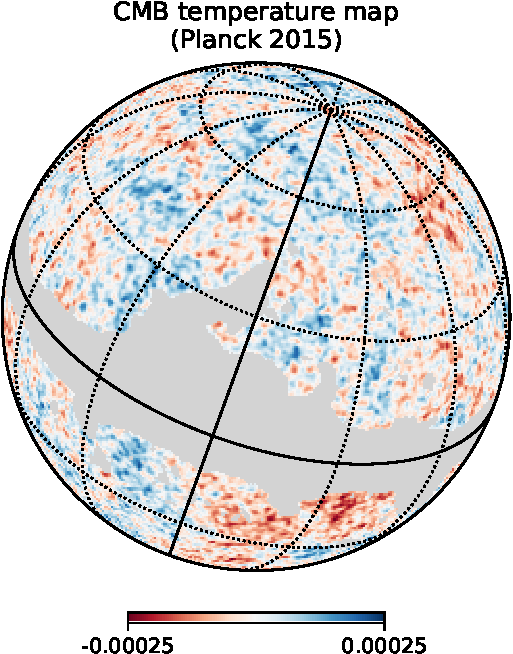
\includegraphics[height=0.25\linewidth]{example_cosmo_cmb}
	\hfill
	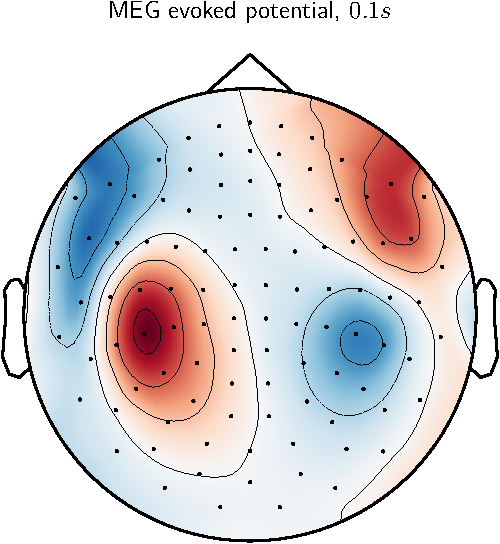
\includegraphics[height=0.25\linewidth]{example_brain_meg}
	\hfill
	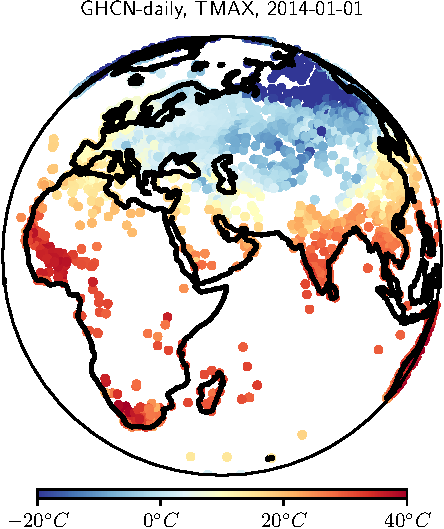
\includegraphics[height=0.25\linewidth]{example_ghcn_daily_tmax}
	\hfill
	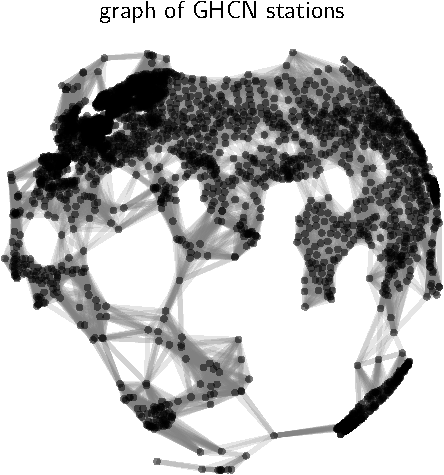
\includegraphics[height=0.25\linewidth]{example_ghcn_graph}
	\caption{
		Examples of intrinsically spherical data: (left) the cosmic microwave background (CMB) temperature from \citet{planck2015overview},
		%with galactic plane masked
		(middle) daily maximum temperature from the Global Historical Climatology Network (GHCN),\protect\footnotemark (right) brain activity recorded through magnetoencephalography (MEG).\protect\footnotemark
		For those examples, a rigid full-sphere pixelization is not ideal: the Milky Way's galactic plane masks observations, brain activity is measured on the scalp only, and the position and density of weather stations is arbitrary and changes over time.
		Graphs can faithfully and efficiently represent sampled spherical data by placing vertices where data has been measured.
		%\todo{something from climate, weather?}
		%\todo{compare ideal full-spheres (like SHREC-17 projection from Esteves, 360 from Coors) to real-world measurements?}
		%\todo{horizontal colorbar for brain}
	}
	\label{fig:examples}
\end{figure}
\footnotetext[1]{\scriptsize\url{https://www.ncdc.noaa.gov/ghcn-daily-description}}
\footnotetext[2]{\scriptsize\url{https://martinos.org/mne/stable/auto_tutorials/plot_visualize_evoked.html}}

Exploit the geometrical properties of the domain, symmetries.

We identify the following desiderata for spherical CNNs:\\
* respect the domain\\
  * rotational equivariance\\
  * deformation (e.g., on the icosahedron for gauge)\\
* powerful / generality $\Rightarrow$ isotropic vs anisotropic\\
* scale: computational cost \& memory usage (feature maps)\\
* flexible (samplings, irregular), simplicity (implementation)\\

Multiple methods have been developed to handle spherical data, each with their strengths and weaknesses.

On the one side, we have Cohen which is computationally very expensive but perfectly equivariant most general, on the other we have cube sphere which computationl very good but not equivariant at all. Other methods are tradedoff between these two. What is a good tradeoff? We think that DeepSphere is

Present the different spherical CNNs with pro and cons $\Rightarrow$ mostly scale vs generality\\
* 2D CNN $\Rightarrow$ doesn't respect geometry and equivariance\\
* Cohen spherical CNN $\Rightarrow$ most general, but doesn't scale\\
* Cohen gauge $\Rightarrow$ fixes scale, at the price of deformation (sphere $\Rightarrow$ icosahedron)\\
* Esteves $\Rightarrow$ ? \\
* Jiang $\Rightarrow$ need a global coordinate system (ok for planets, not projections like cosmo)\\

\begin{table}[b]
    \centering
    \begin{tabular}{l|c|c|c|c}
         method & equivariance & generality & scalability & flexibility \\
         \hline
        Cohen & & & &  \\
         \hline
        Gauge & & & &  \\
         \hline
        Esteves & & & &  \\
         \hline
        Jiang & & & &  \\
         \hline
        2D CNN (cubed sphere) & & & &  \\
         \hline
        Ours & & & &  \\
    \end{tabular}
    \caption{Caption}
    \label{tab:my_label}
\end{table}

This paper focuses on improving the equivariance of \cite{perraudin2019deepsphere}, a scalable graph-based method designed for cosmological applications.
\todo{cite RLGM paper}
Experiments on multiple problems of practical interest shows the competitiveness and flexibility of our method.
Furthermore, those experiments show, contrarily to previously published results \cite{cohen_gauge_2019}, that anisotropic filters may be an unnecessary price to pay.

\section{Method [1 pages]}

* HEALPix: improvement from DeepSphere v1 \cite{perraudin2019deepsphere} \\
* equiangular: Renata \& Pascal \\

\cite{khasanova2017graphomni} designed a discrete Laplacian that is explicitly intended to work on the sphere with the equiangular sampling. They consider the set $\mathcal G$ of all the possible graphs where each node is connected only to four of its nearest neighbours (North, Sud, West, East) and propose a weighting scheme $w_{ij}$ that minimizes the difference in the response to the polynomial spectral filter $\mathcal F = \mathbf L$ evaluated on images of the same object seen at different latitudes. In other words, they solve the minimization problem
\begin{equation} \label{eq:minimization frossard}
	\min_{W\in\mathcal G} \left|\mathcal{F}\left(\mathbf{y}\left(v_{ e}\right)\right)-\mathcal{F}\left(\mathbf{y}\left(v_{ i}\right)\right)\right|
\end{equation}
for the adjacency matrix $W$, where $\mathbf y(v_i)$ is the image of the object on the sphere centered on the vertex $v_i$, and $\mathcal F (\mathbf y(v_e))$ is the response of the filter at the vertex $v_e$ that lies at the same longitude of the vertex $v_i$ but on the equator. In their work they prove that the optimal weights solving the minimization problem (\ref{eq:minimization frossard}) are given by weights $w_{ij}$ inversely proportional to the Euclidean distance between vertices:
\begin{equation} \label{eq:frossard weights}
	w_{ij} = \frac{1}{\norm{x_i-x_j}}
\end{equation}

\begin{figure}
	\centering
	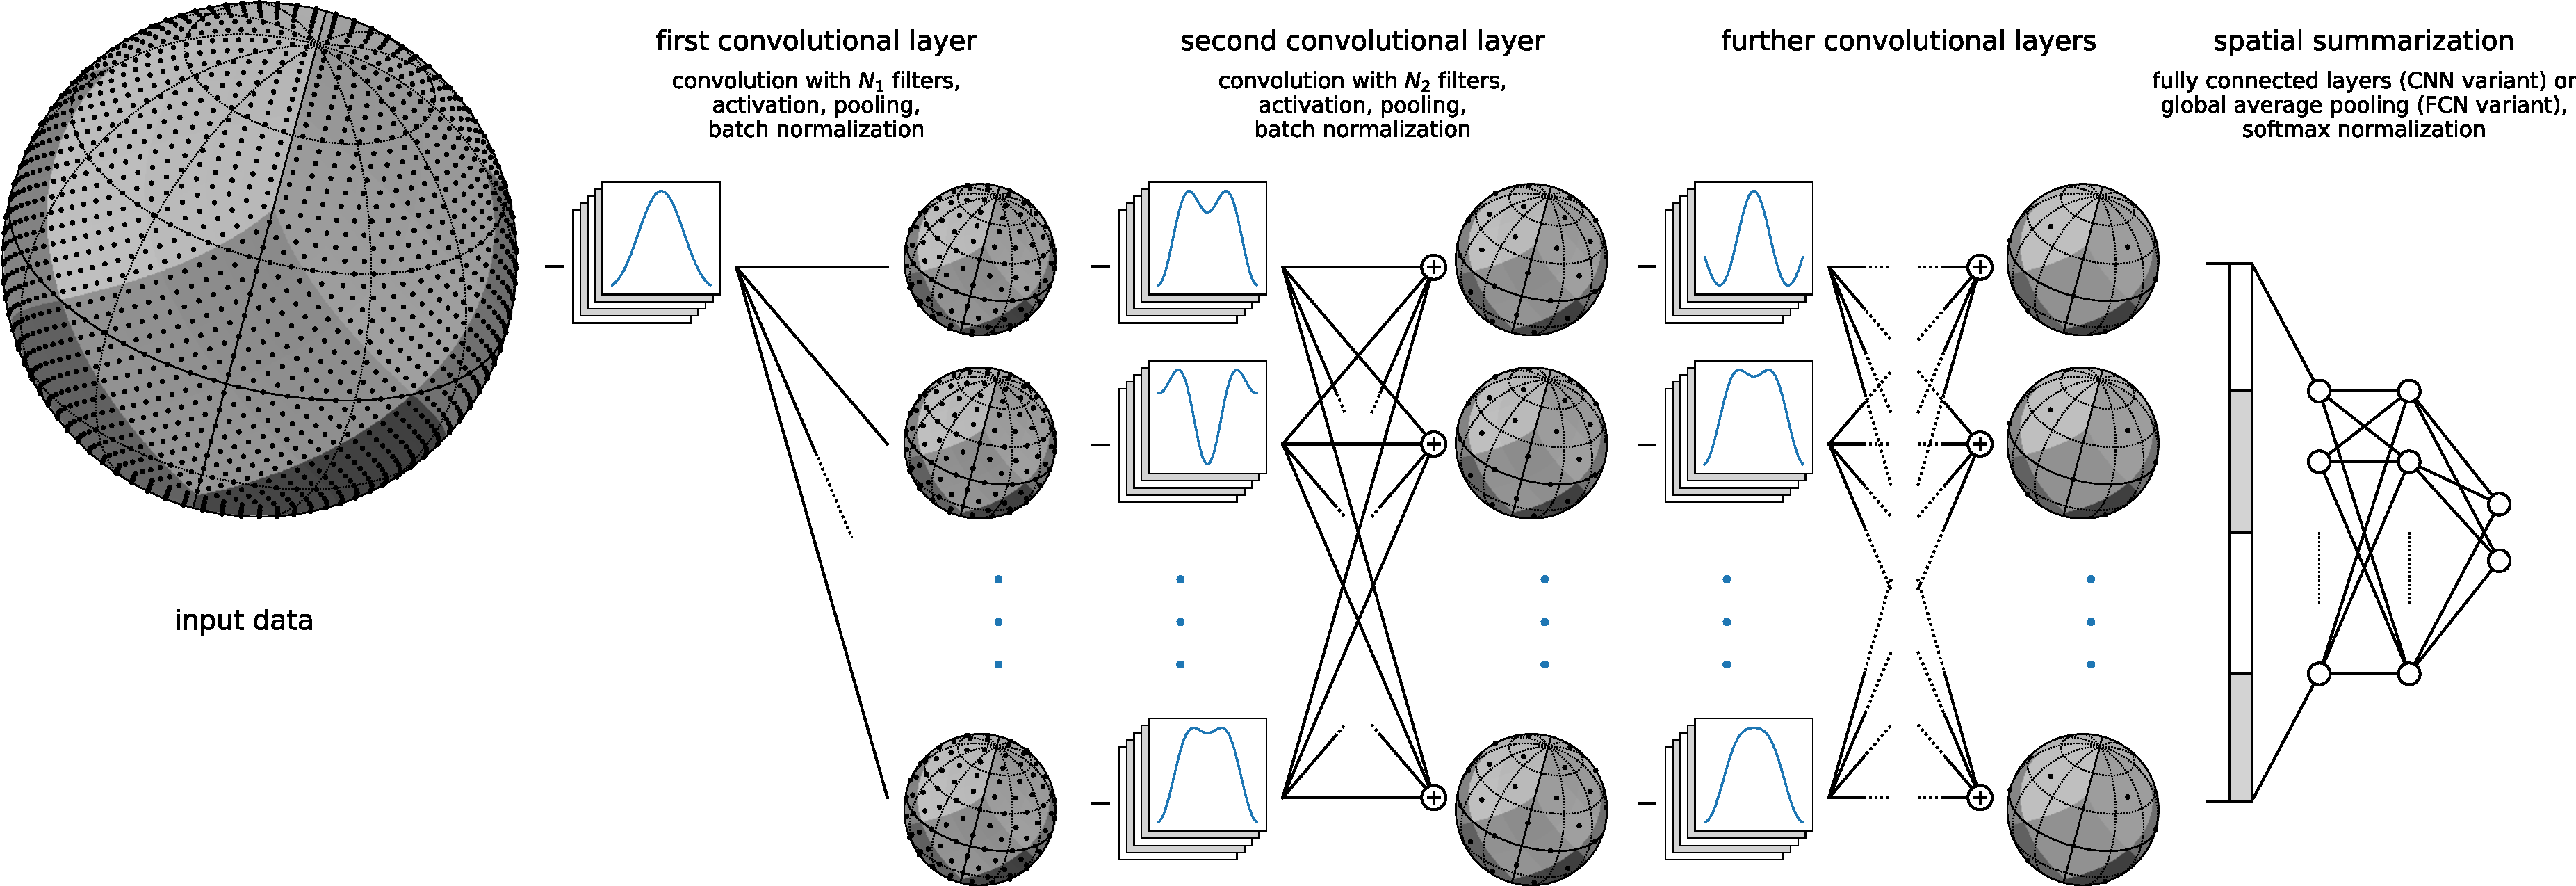
\includegraphics[width=0.9\linewidth]{figure_architecture_v3}
	\caption{Example architecture from \cite{perraudin2019deepsphere}.
		Global tasks need a spatial summarization: the FCN variant is rotation invariant (and accepts inputs of varying sizes), while the CNN variant is not.
		Dense tasks (when the output lives on the sphere, like segmentation) are rotation equivariant.
	}
	\label{fig:architecture}
\end{figure}

\section{Is graph convolution equivariant to rotation? [2 pages]}

% The plan for this section
% 0) Explain why the Laplacian is so important...
By definition, the graph convolution (on the sphere) is rotation equivariant to rotation, if and only if, it commutes with the rotation operator. 
As, in the context of this work, graph convolution can be performed by successive application of the graph Laplacian, i.e: $g(\b{L}) \b{f} = \left(\sum_{i=0}^K \alpha_i \b{L}^i\right) \b{f}$, if the graph Laplacian $\b{L}$ commutes with the rotation operator, then, by recursion, it will also commute with the convolution $g(\b{L})$.
Hence to simplify our analysis, we concentrate on the graph Laplacian.

% 0.5) Explain the sampling and metric
We first need to deal with the sampling problem. 
Take a sampling scheme $V=\{v_i\in\mathbb S^2, i=0, \dots, n\}$ of the sphere, a weighted undirected graph $G(V, E, \mathbf W)$, a signal $f: \mathbb S^2\to\mathbb R$ and its sampled representation $\mathbf f:\ f_i=f(v_i)$. Suppose that there exists a sampling operator $T_V: L^2(\mathbb S^2) \supset F\to \mathbb R^n,\  T_V(f) = \mathbf f$ defined on a suitable subspace $F$ of $L^2(\mathbb S^2)$ such that it is invertible, i.e., we can unambiguously reconstruct the function $f\in F$ from its sampled values $\mathbf f$. The existence of such subspace depends on the sampling scheme $V$, and its characterization is a common problem in signal processing \cite{Driscoll:1994:CFT:184069.184073}. Define the rotation operator $R(g), g\in SO(3)$: $R(g) f(\omega) = f\left(g^{-1} \omega\right)$. 

We now want to understand how to set the edges and the weights of $G$ such that
\begin{equation} \label{eq:equivariance}
	T \R(g) T^{-1} \Omega_k T f = \Omega_k T R(g) f,
\end{equation}
i.e., the graph convolution $\Omega_k$ and any rotation $R(g)$ commute.

Verifying equation (\ref{eq:equivariance}) is really hard in practice, due to the fact that for almost all sampling schemes $V$ it is not known if there exists a space $F$ in which $T$ is invertible. A special case is the \textit{equiangular sampling} scheme where a sampling theorem holds \cite{Driscoll:1994:CFT:184069.184073}, and thus we have a closed form of $T^{-1}$. For sampling schemes where no such sampling theorem is available, there are implementations of discrete SHT to reconstruct a sampled signal $\mathbf f$, thus providing a way to approximate $T^{-1}$. Thanks to this we are able, for a given sampling, a given function $f$, a given rotation $g$, and a given kernel $k$, to compute the \textit{normalized equivariance error}
\begin{equation} \label{eq:equivariance error}
	E_{G}(f, g) = \left(\frac{ \norm {T R(g) T^{-1} \Omega_k Tf - \Omega_k T R(g) f}_{L^2(\mathbb R^2)}}{\norm {Tf}_{L^2(\mathbb R^2)}}\right)^2,
\end{equation}
where $T^{-1}$ is substituted with a discrete SHT in case $T$ is not invertible.
A measure of how equivariant a graph is with respect to rotations will then be given by the \textit{mean equivariance error}
\begin{equation} \label{eq:mean equivariance error}
	\overline E_G = \mathbb E_{f, g} \ E_G(f, g).
\end{equation}
In practice the expected value is obtained by averaging over a finite number of random functions and random rotations. The mean equivariance error $\overline E_G$ gives us an indication of how close the graph $G$ is from being equivariant to rotations. 
Of course result will depend on the sampling and on the graph construction.

% !) summary the work of Khasanova -> No! to be put in section 2) Method

% 2) explain our approach
We inspire ourselves with Belkin, which says that for \emph{uniform sampling} the graph Laplacian converges toward the Laplace-Beltrami. b) The Laplace Beltrami commute with rotation. The following theorem extend the work of Belkin and Nyiogi to fixed sampling \nati{(Including Healpix or not?)}. 
Given a sampling $V = \{x_0, \dots, x_{n-1}\}$ define $\sigma_i$ to be the patch of the surface of the sphere corresponding to $x_i$, define $A_i$ to be its corresponding area and $d_i$ to be the radius of the smallest ball in $\mathbb R^3$ containing $\sigma_i$. Define $d^{(n)} := \max_{i=0, \dots, n}d_i$ and $A^{(n)}=\max_{i=0, \dots, n}A_i$.

\begin{theorem}
	For a sampling $\mathcal P = \{x_i\in\mathbb S^2\}_{i=0}^{n-1}$ of the sphere that is equi area and such that $d^{(n)} \leq \frac{C}{\sqrt{n}}$, for all $f: \mathbb S^2 \rightarrow \mathbb R$ Lipschitz with respect to the euclidean distance in $\mathbb R^3$, for all $y\in\mathbb S^2$, there exists a sequence $t_n = n^\beta$ such that the rescaled Heat Kernel Graph Laplacian operator $\frac{|\mathbb S^2|}{4\pi t_n}L^t_n$ converges pointwise to the Laplace Beltrami operator on the sphere $\triangle_{\mathbb S^2}$  for $n\to\infty$:
	$$ \lim_{n\to\infty}\frac{|\mathbb S^2|}{4\pi t_n} L_n^{t_n}f(y) =  \triangle_{\mathbb S^2}f(y).$$
	\label{theo:pointwise convergence for a regular sampling}
\end{theorem}

This is \emph{not} a proof of equivariance of the graph convolution for a specific sampling. We simply observe that the graph Laplacian converges pointwisely toward an operator that commutes with rotation. To have the desired equality in eq..., we would need to prove a stronger result, for example uniform convergence (in the space of the operators).
\nati{Should we put this here?: }This does not hold in general \cite{belkin-spectral}. However, we believe that this is achievable for a bandlimited signals.
More importantly, the proof of theorem \ref{theo:pointwise convergence for a regular sampling} in Appendix ... inspires us in the construction of our graph Laplacian. a) use gaussian kernel b) we need to adjust t with respect of n such that ...

% 3) Show experimental results
Define the error, show results and comments
\begin{figure}
	\centering
	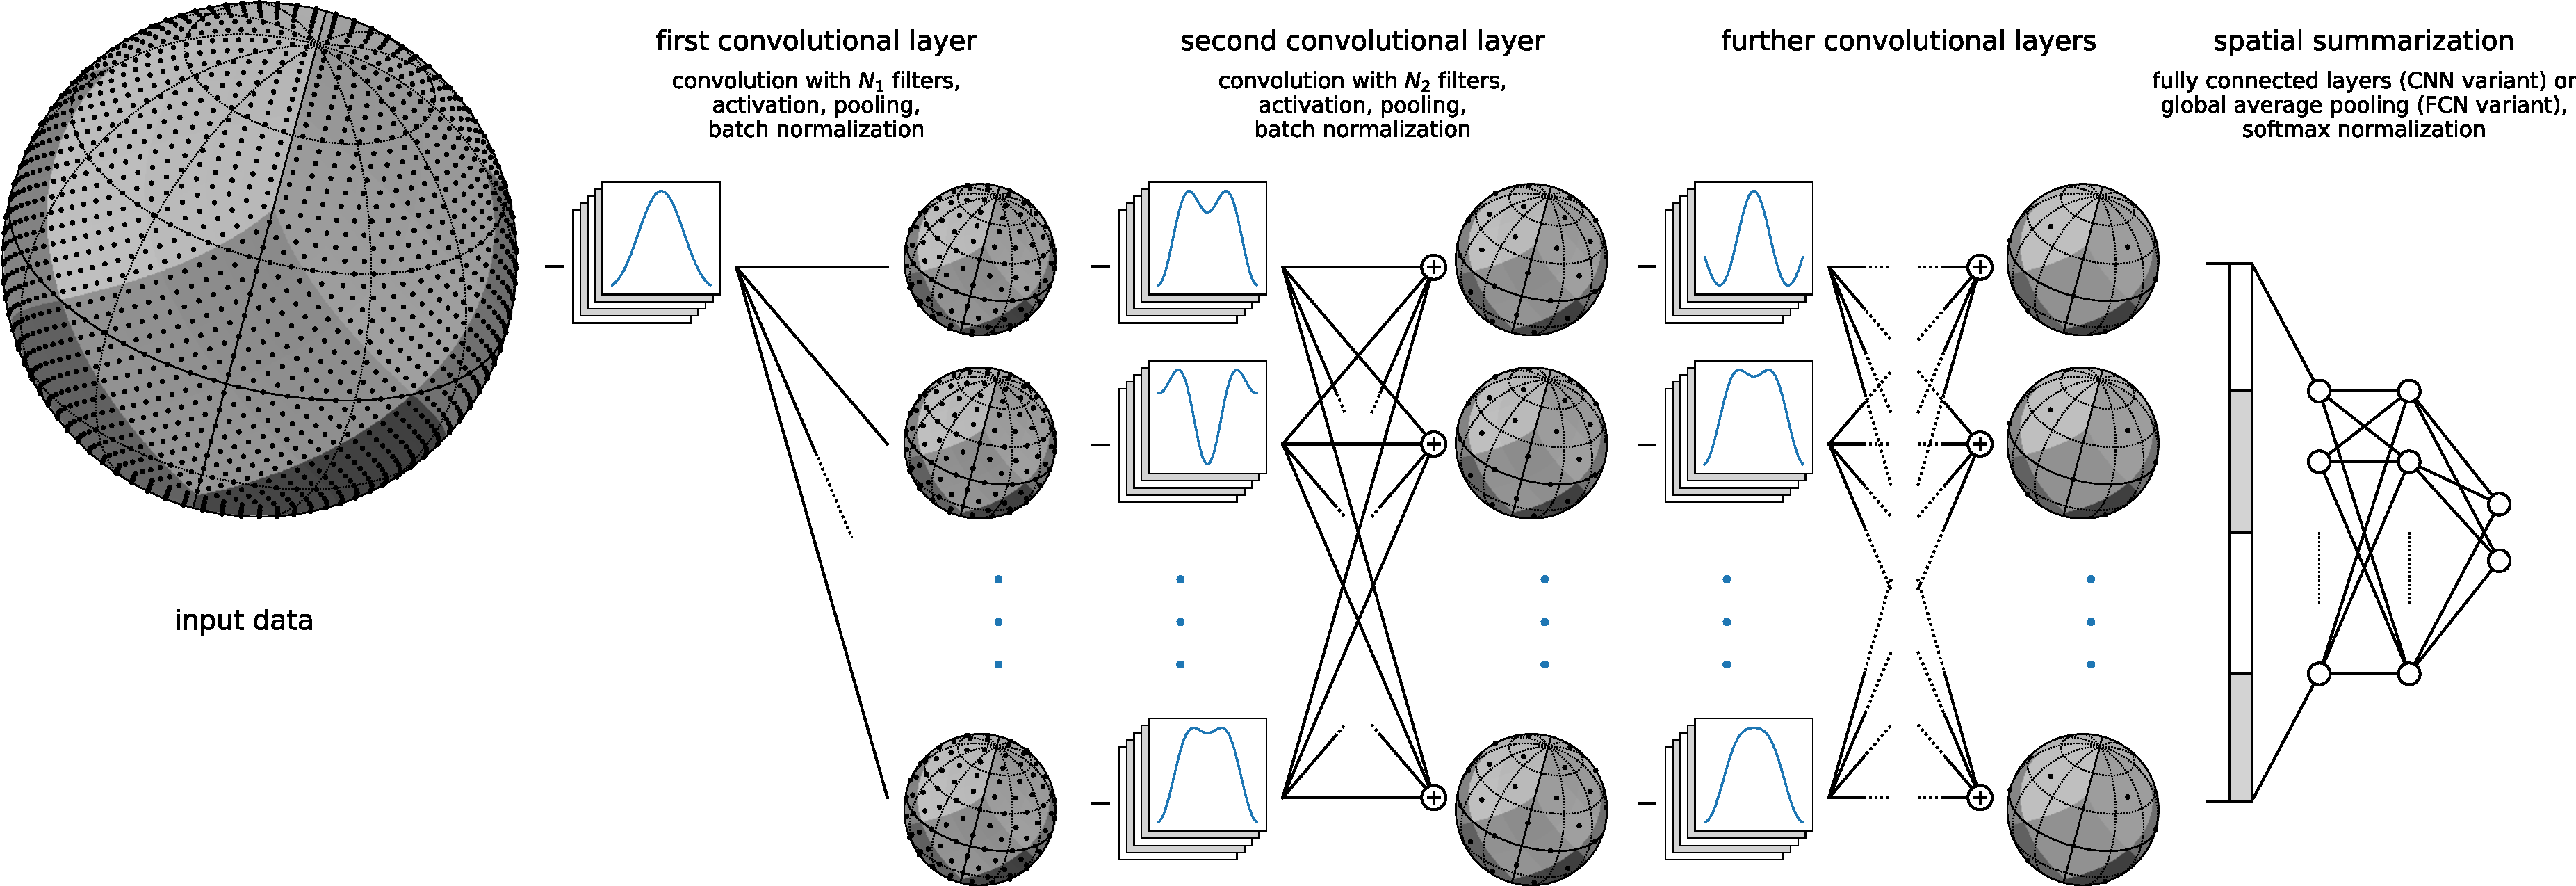
\includegraphics[width=0.9\linewidth]{figure_architecture_v3}
	\caption{Example architecture from \cite{perraudin2019deepsphere}.
		Global tasks need a spatial summarization: the FCN variant is rotation invariant (and accepts inputs of varying sizes), while the CNN variant is not.
		Dense tasks (when the output lives on the sphere, like segmentation) are rotation equivariant.
	}
	\label{fig:architecture}
\end{figure}


Explain the difference of errors... Uniform sampling is better

\section{Experiments [2 pages]}

\todo{
Show: \\
* meet the desiderata \\
* DeepSphere V1 and V2 are equivalent in practice, wait on SHREC and cosmo exp \\
* anisotropy doesn't help \\
}

\subsection{3D objects recognition}

\todo{
* same perf as other spherical CNNs, but 40 times faster \\
* compare samplings (equi, HEALPix) $\Rightarrow$ not much difference \\
* compare with improved graph (Nside=32) $\Rightarrow$ no improvement as information in the low frequencies (PSD, and works down to nside=8) \\
* ModelNet 40: same conclusions $\Rightarrow$ appendix \\
}

\begin{table}
    \centering
    \begin{tabular}{l|c c c c c}
        \multicolumn{1}{l}{} & \multicolumn{2}{c}{performance} & \multicolumn{1}{c}{size} & \multicolumn{2}{c}{speed}\\
        \cmidrule(lr){2-3} \cmidrule(lr){4-4} \cmidrule(lr){5-6}
        \multicolumn{1}{l}{Method} & F1 & mAP & params & inference [ms] & training \\ \hline
        \cite{cohen_spherical_2018} & 78.85 & 67.6 & 1.4M & 38 & 50h\\
        % Cohen \emph{s2cnn\_simple} & 78.59 & 78.85 & 400k & 12ms & 32h\\
        \cite{esteves_learning_2017} & 79.36 & 68.5 & 500k & 10 & 2h52\\ \hline
        DeepSphere \emph{Equiangular} & 79.36 & 66.5 & 190k & 1 & 50m \\
        DeepSphere \emph{HEALPix} & 80.65 & 68.6 & 190k & 1 & 50m\\
        DeepSphere \emph{Improved HEALPix} & ? & ? & 190k & ? & ?
    \end{tabular}
    \caption{Performance of different models for SHREC'17 task. F1-score computed with sklearn, mAP from the official script of the competition.}
    \label{tab:SHREC17_class}
\end{table}

* inference speed = time for a single instance to do a single training pass\\
* training speed = time for the neural net to train to peak performance\\

* diminish resolution $\Rightarrow$ no change in result until nside=8, no change for high resolution $\Rightarrow$ info in the low freq\\
* same conclusion, anisotropy unnecessary cost to pay\\
* Limited by representation of data? yep, treat them as point clouds \\

\subsection{Cosmological model discrimination}

\todo{
* other sphercial CNNs cannot scale to 10M pixels (tested on 10k at most) \\
* redo the experiment with the optimal graph \\
}

\subsection{Climate event detection}

* small: better perf than gauge and Jiang. due to icosahedron distortion? to be confirmed\\
* cannot compare with Mudigonda (16 vs 1 input channel)\\
* (full: we scale (50B pixels, 20TB) $\Rightarrow$ lead to better perf?) \\

\begin{table}
	\begin{tabular}{l|c c c c}
	\multicolumn{1}{l}{} & Accuracy & Average Precision & \multicolumn{2}{c}{Speed}\\
	\cmidrule(lr){2-2} \cmidrule(lr){3-3} \cmidrule(lr){4-5}
	\multicolumn{1}{l}{Method} & mean & mean & inference [ms] & training \\ \hline
	%Mudigonda et al. & 97 & 74 & 65 & 78.67 & - & - & - \\
	\cite{jiang_spherical_2019} & 94.67 & - & - & -\\
	\cite{jiang_spherical_2019} \emph{rerun} & 94.95 & 38.41 & 10 & 10h\\
	% 328'339
	\cite{cohen_gauge_2019} (S2R) & 97.5 & 68.6 & - & -\\
	\cite{cohen_gauge_2019} (R2R) & 97.7 & 75.9 & - & -\\ \hline
	% unknown
	DeepSphere (weighted) & $97.8\pm 0.3$ & $77.15\pm 1.94$ & 33 & 13h \\
	DeepSphere (non-weighted) & $87.8\pm 0.5$ & $89.16\pm 1.37$ & 33 & 13h\\
	% 12'926'432
	\end{tabular}
	\caption{Climate pattern segmentation mean accuracy (\%), mean Average Precision (\%) and speed for different models run on the icosahedron dataset from \cite{jiang_spherical_2019}}
\end{table}

* Jiang rerun with a batch size of 64 instead of 256 due to memory limit.\\
* cross entropy loss between parenthesis\\
* 5 runs for each loss to obtain mean and std\\

* trade off between AP and accuracy in the case of TC class, it seems.\\
* change base, influence?\\

* full dataset not enough memory to run a correct model

% jiang like correct: 99.81631631, 13.18655162, 52.62412867, 55.20899887;  0.3990812 , 0.80056251, 0.59982186; 4 ms; 2h40
% more feat: 99.67871329, 38.78607557, 66.37910064, 68.2812965: 0.99981102, 0.60714174, 0.83236147, 0.71975161; 12ms; 6h20

\subsection{GHCN}

* task is artificial, but it shows DeepSphere's flexibility\\
* structure (looking around) help for prediction\\

* non-regular sampling with different density over the globe (continent vs ocean)\\
* resulting graph is not rotation equivariant\\
* Two different tasks: a dense regression and a global regression\\

\paragraph*{dense regression - future temperature estimation}~\\
* Task is to find the temperature at day T, knowing the temperature of the 5 previous days.\\
* Goal is to change the order of the chebyshev filter to find the influence of the structure.\\
* order 0 is the same as time series, as the pixel have no information of its neighborhood.\\
* increasing order is good until threshold.\\
* The NN indeed predicts the correct temperature at day T, and not day T-1 (baseline) even though there is small difference.\\



\paragraph*{global regression - day in year estimation}~\\
* days represented by a sine to represent the periodic nature of the year.\\
* task too easy, temperature feature already periodic $\Rightarrow$ second experiment with only precipitation feature\\
* structure is still helping\\

\begin{table}
    \centering
    \begin{tabular}{c|ccc}
        order & future temp & day (temperature) & day (precipitations) \\ \hline
        0 & 0.896 & 0.881 & - 0.920\\
        4 & 0.919 & 0.969 & 0.597\\
    \end{tabular}
    \caption{R2 coefficient for different tasks on the GHCN dataset}
    \label{tab:GHCN_results}
\end{table}



\section{Conclusion [0.5 pages]}

* DeepSphere seems to be in the sweet spot of tradeoffs. Recall the desiderata.\\
  * respect geometry: No need for a very precise equivariance, i.e., a very good graph...\\
  * Not the most general (restricted to isotropic filters), but didn't hurt perf in any experiment\\
  * scales linearly $\Rightarrow$ cannot do better ($n^{1.25}$ for best HEALPix, linear for not optimal)\\
  * flexible $\Rightarrow$ independent of the sampling\\

future work:\\
* when anisotropy useful? (research question)\\
* irregular sampling while respecting the geometry\\
* beyond the sphere, any manifold\\

\newpage
\subsubsection*{Author Contributions}
Left blank for anonymity reason
% If you'd like to, you may include  a section for author contributions as is done
% in many journals. This is optional and at the discretion of the authors.

\subsubsection*{Acknowledgments}
Left blank for anonymity reason
% Use unnumbered third level headings for the acknowledgments. All
% acknowledgments, including those to funding agencies, go at the end of the paper.

\bibliography{references}
\bibliographystyle{iclr2020_conference}

\newpage
{\LARGE \sc {Supplementary Material}}
\appendix

\section{Proof of theorem}

\begin{definition}{}(Heat Kernel Graph Laplacian operator)\\
	\label{def:Heat Kernel Graph Laplacian operator}
	\text{Given a sampling $\{x_i\in\mathcal M\}_{i=0}^{n-1}$ of the manifold we define the \textbf{operator} }$L_n^t$ such that
	$$L_n^tf(y) := \frac{1}{n}\left[ \sum_{i=0}^{n-1} \exp{-\frac{||x_i-y||^2}{4t}}\left(f(y)-f(x_i)\right)\right]$$
\end{definition}
\begin{definition}{} \cite{Belkin:2005:TTF:2138147.2138189}\\ \label{eq: my L^t} Let $\mu$ be the uniform probability measure on the manifold $\mathcal M$, and let $\text{vol}(\mathcal M)$ be the volume of $\mathcal M$. We define the functional approximation to the Laplace-Beltrami operator to be the operator $L^t: L^{2}(\mathcal{M}) \rightarrow L^{2}(\mathcal{M})$ such that
	\label{def:Functional approximation to the Laplace-Beltrami operator}
	$$ L^tf(y) = \int_{\mathcal M}e^{-\frac{||y-x||^2}{4t}}\left(f(y)-f(x)\right)d\mu(x)$$
\end{definition}

The core of the work of Belkin et al. is the proof, that we will not discuss, of the following proposition.

\begin{prop} \cite{Belkin:2005:TTF:2138147.2138189} \\
Let $\mathcal M$ be a $k$-dimensional compact smooth manifold embedded in some euclidean space $\mathbb R^N$, and fix $p\in\mathcal M$. Let the data points $x_1, \dots, x_n$ be sampled form a uniform distribution on the manifold $\mathcal M$. Set $t_n=n^{-\frac{1}{k+2+\alpha}}$, for any $\alpha>0$ and let $f\in\mathcal C_\infty(\mathcal M)$. Then
	$$\frac{1}{t}\frac{1}{(4\pi t)^{k/2}} L^tf(p) \xrightarrow{t\to 0 } \frac{1}{\text{vol}(\mathcal M)}\triangle_{\mathcal M}f(p).$$
	\label{prop:3}
\end{prop}

Our first goal is to prove the following Proposition:
\vspace{0.5cm}
\begin{prop}\label{prop:1}
	For an equal area sampling $\{x_i\in\mathbb S^2\}_{i=0}^{n-1}: A_i=A_j \forall i,j$ of the sphere it is true that for all $f: \mathbb S^2 \rightarrow \mathbb R$ Lipschitz with respect to the euclidean distance $||\cdot||$ with Lipschitz constant $\mathcal L_f$
	$$
	\left| \int_{\mathbb S^2}f({ x})\text{d}{\mu(x)} - \frac{1}{n}\sum_i f( x_i)\right|\leq \mathcal L_fd^{(n)}.
	$$
	Furthermore, for all $y\in\mathbb S^2$ the Heat Kernel Graph Laplacian operator $L^t_n$ converges pointwise to the functional approximation of the Laplace Beltrami operator $L^t$
	$$ L_n^tf(y)\xrightarrow{n\to\infty} L^tf(y).$$
\end{prop}
\vspace{0.5cm}

\begin{proof}

	Let us assume that the function $f:\mathbb R^3\rightarrow \mathbb R$ is Lipschitz with Lipschitz constant $\mathcal L_f$, we have

	$$\left| \int_{\sigma_{i}}f({ x})\text{d}{\mu(x)} - \frac{1}{n}f( x_i)\right| \leq \mathcal L_fd^{(n)}\frac{1}{n} $$

	So, by triangular inequality and by summing all the contributions of all the $n$ patches
	$$\left| \int_{\mathbb S^2}f({ x})\text{d}{\mu(x)} - \frac{1}{n}\sum_i f( x_i)\right| \leq \sum_i \left| \int_{\sigma_{i}}f({ x})\text{d}{\mu(x)} - \frac{1}{n}f( x_i)\right|\leq n  \mathcal L_fd^{(n)}\frac{1}{n} = \mathcal L_fd^{(n)}$$
	Thanks to this result, we have the following two pointwise convergences

	$$\forall f \text{ Lipschiz,}\quad \forall y\in\mathbb S^2,  \quad\quad \frac{1}{n}\sum_i e^{-\frac{||x_i-y||^2}{4t}}\rightarrow \int e^{-\frac{||x-y||^2}{4t}}d\mu(x)$$
	$$\forall f \text{ Lipschiz,}\quad \forall y\in\mathbb S^2,  \quad\quad \frac{1}{n}\sum_i e^{-\frac{||x_i-y||^2}{4t}}f(x_i)\rightarrow \int e^{-\frac{||x-y||^2}{4t}}f(x)d\mu(x)$$

	Definitions \ref{def:Heat Kernel Graph Laplacian operator} and \ref{def:Functional approximation to the Laplace-Beltrami operator} end the proof.
\end{proof}
\vspace{0.5cm}

Now, we just proved that \textit{keeping t fixed} $L_n^tf(x)\rightarrow L^tf(x)$. Now our goal is to prove that:

\vspace{0.5cm}
\begin{prop}\label{prop:2}
	Given a sampling regular enough, i.e., for which we assume $A_i=A_j \ \forall i,j\text{ and }d^{(n)}\leq \frac{C}{\sqrt{n}}$, for a fixed $t>0$, a fixed Lipschitz function $f$ and a fixed point $y\in\mathbb S^2$ there exists a sequence $t_n = n^\beta, \beta<0$ such that
$$
\forall f \text{ Lipschitz, } \forall x\in\mathbb S^2 \quad \left|\frac{1}{4\pi t_n^2}\left(L_n^{t_n}f(x) - L^{t_n}f(x)\right)\right|\xrightarrow{n\to \infty}0.
$$
\end{prop}
\vspace{0.5cm}

The main result of this section, theorem  \ref{theo:pointwise convergence in the healpix case}, is then an immediate consequence of Proposition \ref{prop:2} and Proposition \ref{prop:3}.

\begin{proof}[Proof of Proposition \ref{prop:2}]

We define for simplicity of notation
\begin{align}
	\phi^t(x;y) &:= e^{-\frac{||x-y||^2}{4t}}\left(f(y)-f(x)\right)\\
	K^t(x,y) &:=  e^{-\frac{||x-y||^2}{4t}}
\end{align}
We start by writing the following chain of inequalities
\begin{align*}
	||L_n^tf-L^tf||_\infty &= \max _{y\in \mathbb S^2} \left|L_n^tf(y)-L^tf(y)\right|\\
	&= \max _{y\in \mathbb S^2} \left| \frac{1}{n} \sum_{i=1}^n \phi^t(x_i; y)- \int_{\mathbb S^2} \phi^t(x;y)d\mu(x) \right|\\
	&\leq \max _{y\in \mathbb S^2}  \sum_{i=1}^n   \left| \frac{1}{n}  \phi^t(x_i; y)- \int_{\sigma_i} \phi^t(x;y)d\mu(x) \right|\\
	&\leq  \max _{y\in \mathbb S^2} \left[\mathcal L_{\phi^t_y}d^{(n)} \right]\\
\end{align*}
where $\mathcal L_{\phi^t_y}$ is the Lipschitz constant of $x \rightarrow \phi^t(x, y)$ and where we used for the last inequality Proposition \ref{prop:1}. If we assume $d^{(n)}\leq \frac{C}{\sqrt{n}}$ we have that

$$||L_n^tf-L^tf||_\infty  \leq  \max _{y\in \mathbb S^2} \left[ \mathcal L_{\phi^t_y} \frac{C}{\sqrt{n}} \right]$$

Let's now find the explicit dependence $t\rightarrow \mathcal L_{\phi^t_y}$
\begin{align*}
	\mathcal L_{\phi^t_y} &= ||\partial_x\phi^t(\cdot;y)||_\infty\\&
	= ||\partial_x\left(K^t(\cdot;y)f\right)||_\infty\\&
	= ||\partial_x K^t(\cdot;y)f + K^t(\cdot;y)\partial_x f||_\infty\\&
	\leq ||\partial_x K^t(\cdot;y)f||_\infty + ||K^t(\cdot;y)\partial_x f||_\infty\\&
	\leq  ||\partial_x K^t(\cdot;y)||_\infty||f||_\infty + ||K^t(\cdot;y)||_\infty||\partial_x f||_\infty\\&
	= ||\partial_x K^t(\cdot;y)||_\infty||f||_\infty + ||\partial_x f||_\infty\\&
	= \mathcal L_{K^t_y} ||f||_\infty + ||\partial_xf||_\infty\\&
	= \mathcal L_{K^t_y} ||f||_\infty + \mathcal L_f
\end{align*}
where $\mathcal L_{K^t_y}$ is the Lipschitz constant of $x\rightarrow K^t(x;y)$. We can observe that such constant does not depend on $y$:

$\mathcal L_{K^t_y} = \norm{\partial_x e^{-\frac{x^2}{4t}}}_\infty = \norm{\frac{x}{2t}e^{-\frac{x^2}{4t}}}_\infty = \left. \frac{x}{2t}e^{-\frac{x^2}{4t}}\right|_{x=\sqrt{2t}}=(2et)^{-\frac{1}{2}}\propto t ^ {-\frac{1}{2}}$

So we can continue
$$\begin{aligned}
	\max _{y\in \mathbb S^2} \left[  \mathcal L_{\phi^t_y} \frac{C}{\sqrt{n}} \right]
	&\leq  \frac{C}{\sqrt{n}} \left( (2et)^{-\frac{1}{2}} \norm{f}_\infty + \mathcal L_f \right)\\
	&\leq \frac{C\norm{f}_\infty}{\sqrt{n}(2et)^{1/2}} +   \frac{C}{\sqrt{n}}\mathcal L_f\\
\end{aligned}$$
So we have that, rescaling by a factor $\frac{1}{4\pi t^2}$
\begin{align*}
	\norm{\frac{1}{4\pi t^2}\left(L_n^tf-L^tf\right)}_\infty&\leq \frac{1}{4\pi t^2}\norm{\left(L_n^tf-L^tf\right)}_\infty \\
	&\leq \frac{C}{4\pi}\left[\frac{\norm{f}_\infty}{\sqrt{2e}}\frac{1}{\sqrt{n}t^{5/2}} + \frac{\mathcal L_f}{\sqrt{n}t^2}\right]
\end{align*}

we want $\begin{cases}
t \rightarrow 0\\
n \rightarrow \infty\\
\sqrt{n}t^{5/2} \rightarrow \infty\\
\sqrt{n}t^2 \rightarrow \infty
\end{cases}$ in order for $ \frac{C}{4\pi}\left[\frac{\norm{f}_\infty}{\sqrt{2e}}\frac{1}{\sqrt{n}t^{5/2}} + \frac{\mathcal L_f}{\sqrt{n}t^2}\right] \xrightarrow[t\to 0 ]{n\to\infty}0$

This is true if $\begin{cases}
t(n) = n^\beta, &\beta\in(-\frac{1}{5}, 0) \\
t(n) = n^\beta, &\beta\in(-\frac{1}{4}, 0)
\end{cases} \implies t(n) = n^\beta, \quad \beta\in(-\frac{1}{5}, 0)$

Indeed

$\sqrt{n}t^{5/2}=n^{5/2\beta+1/2}\xrightarrow{n \to \infty} \infty$ since $\frac{5}{2}\beta+1/2>0 \iff \beta>-\frac{1}{5}$

$\sqrt{n}t^2=n^{2\beta+1/2}\xrightarrow {N \to \infty} \infty$ since $2\beta+1/2>0 \iff \beta>-\frac{1}{4}$

So, for $t=n^\beta$ with $\beta\in(-\frac{1}{5}, 0)$ we have that

$$\begin{cases}
(t_n)\xrightarrow{n\to\infty}0\\
\norm{\frac{1}{4\pi t_n^2}L_n^{t_n}f-\frac{1}{4\pi t_n^2}L^{t_n}f}_\infty  \xrightarrow{n\to\infty}0
\end{cases}$$

\end{proof}

The proof of theorem \ref{theo:pointwise convergence in the healpix case} is now trivial:
\begin{proof}[Proof of Theorem \ref{theo:pointwise convergence in the healpix case}]
	Thanks to Proposition \ref{prop:2} and Proposition \ref{prop:3}	we conclude that $\forall y\in\mathbb S^2 $
	$$\lim_{n\to\infty}\frac{1}{4\pi t_n^2} L_n^{t_n}f(y) =  \lim_{n\to\infty}\frac{1}{4\pi t_n^2} L^{t_n}f(y) = \frac{1}{|\mathbb S^2|}\triangle_{\mathbb S^2}f(y) $$
\end{proof}

The proof of this result is instructive since it shows that we need to impose some regularity conditions on the sampling. If the sampling is equal area as HEALPix, meaning that all the patches $\sigma_i$ have the same area, then we need to impose that $ d^{(n)}\leq \frac{1}{\sqrt{n}}$. If the sampling is not equal area, meaning that in general $A_i\neq A_j$, it can be shown that we need a slightly more complex condition: $\max_{i=0,\dots,n-1}d_iA_i\leq Cn^{-\frac{3}{2}}$.\\
In the work of Belkin et al. \cite{Belkin:2005:TTF:2138147.2138189} the sampling is drawn form a uniform random distribution on the sphere, and their proof heavily relies on the uniformity properties of the distribution from which the sampling is drawn. In our case the sampling is deterministic, and the fact that for a sphere there doesn't exist a regular sampling with more than 12 points (the vertices of a icosahedron) is indeed a problem that we need to overcome by imposing the regularity conditions above.

To conclude, we can see that the result obtained has the same form than the result obtained in \cite{Belkin:2005:TTF:2138147.2138189}. Given the kernel density $t(n)=n^\beta$, if Belkin et al. proved convergence in the random case for $\beta \in (-\frac{1}{4}, 0)$, we proved convergence in the HEALPix case for $\beta \in (-\frac{1}{5}, 0)$. This kind of result can be interpreted in the following way. In order to have this pointwise convergence, we need to reduce the kernel width but \textit{not so fast} compared to the resolution of the graph. In other words, the kernel width has to be reduced but is somewhat limited by the resolution of the graph. In the next section we'll see how to set in practice a good kernel width $t$ given a graph resolution $n$.
\begin{remark}
	Pointwise convergence is just a necessary condition for spectral convergence.  Theorem \ref{theo:pointwise convergence in the healpix case} does not imply convergence of eigenvalues and eigenvectors.
\end{remark}

\section{Experimental details}

* Network architecture and details

\subsection{3D object Recognition}
\subsubsection*{Detailed results}
\paragraph*{SHREC17}

\begin{table}
    \centering
    \begin{tabular}{l|c c r r}
        \multicolumn{1}{l}{} & \multicolumn{2}{c}{performance} & \multicolumn{2}{c}{speed}\\
        \cmidrule(lr){2-3} \cmidrule(lr){4-5}
        \multicolumn{1}{l}{Method} & Accuracy & F1-score & inference & training \\ \hline
        Cohen \emph{s2cnn} & - & - & 38ms & 50h\\
        % Cohen \emph{s2cnn\_simple} & 78.59 & 78.85 & 400k & 12ms & 32h\\
        Esteves \emph{sphericalcnn} & 79.18 & 79.36 & 9.8ms & 2h52\\ \hline
        DeepSphere \emph{Equiangular} & 79.25 & 79.36 & 0.9ms & 47m \\
        DeepSphere \emph{HEALPix} & 80.42 & 80.65 & 0.9ms & 46m\\
        DeepSphere \emph{Improved HEALPix} & 80.76 & & &
    \end{tabular}
    \caption{Performance of different models}
    \label{tab:SHREC17_class}
\end{table}

\begin{table}
    \centering
    \begin{tabular}{l|c c c c|c c c c}
     & \multicolumn{4}{c|}{micro (label average)} & \multicolumn{4}{c}{macro (instance average)} \\
    Method & P@N & R@N & F1@N & mAP & P@N & R@N & F1@N & mAP \\ \hline
    Cohen \emph{s2cnn} & 0.701 & 0.711 & 0.699 & 0.676 & - & - & - & - \\
    % Cohen \emph{s2cnn\_simple} & 0.704 & 0.701 & 0.696 & 0.665 & 0.430 & 0.480 & 0.429 & 0.385\\
    Esteves \emph{sphericalcnn} & 0.717 & 0.737 & - & 0.685 & 0.450 & 0.550 & - & 0.444\\ \hline
    DeepSphere \emph{Equiangular} & 0.709 & 0.700 & 0.698 & 0.665 & 0.439 & 0.489 & 0.439 & 0.403 \\
    DeepSphere \emph{HEALPix} & 0.725 & 0.717 & 0.715 & 0.686 & 0.475 & 0.508 & 0.468 & 0.428\\
    DeepSphere \emph{Improved HEALPix} & & & & &
    \end{tabular}
    \caption{Performance of different models over SHREC17 perturbed dataset as a retrieval task, using the official script of the competition.}
    \label{tab:SHREC17_retriev}
\end{table}

\paragraph*{ModelNet 40}

\begin{table}
    \centering
    \begin{tabular}{c|cccc}
         &  x/x & z/z & SO3/SO3 & z/SO3 \\ \hline
Cohen & 85.0 & - & - & - \\
Jiang & 90.5 & - & - & - \\
Esteves \emph{scnn} & - & 88.9 & 86.9 & 78.6 \\
%Esteves \emph{MVCNN} & 94.69 & - & - & - \\
DeepSphere & 87.8 & 86.8 & 86.7 & 76.9
    \end{tabular}
    \caption{Accuracy (in percent) on test set, for different models. The x dataset has no augmentation, the z dataset is augmented with rotation around Z-axis, and SO3 with ZYZ rotations.}
    \label{tab:mn40_results}
\end{table}

\subsubsection*{HEALPix}

HEALPix sampling, input signal at Nside = 32

CNN having 5 convolutional layers, a global average pooling layer and a fully-connected layer at the end, such as this:
\begin{dmath}
    [GC_{16}\, +\, BN\, +\, ReLU]_{nside32}\, +\, \textrm{Pool}\, +\, [GC_{32}\, +\, BN\, +\, ReLU]_{nside16}\, +\, \textrm{Pool}\, +\, [GC_{64}\, +\, BN\, +\, ReLU]_{nside8}\, +\, \textrm{Pool}\, +\, [GC_{128}\, +\, BN\, +\, ReLU]_{nside4}\, +\,\textrm{Pool}\, +\, [GC_{256}\, +\, BN\, +\, ReLU]_{nside2}\, +\, \textrm{Pool}\, +\, GAP\, +\, FCN\, +\, \textrm{softmax}
\end{dmath}
Each convolutional layer has a graph convolution using Chebyshev polynomial approximation, batch normalization and ReLU activation. The order of the Chebyshev polynomial is 4 for each layer, the number of feature maps are [16, 32, 64, 128, 256] respectively and down-sampling to the immediate smaller resolution for each layer.

number of parameter: 190k TODO exact number?

batch size 32, adam optimizer, constant learning rate of $5 \cdot 10^{-2}$
cross-entropy loss, and add triplet loss from ``Esteves et al.''

30 epochs with augmented dataset, 3 random translation perturbation, or 90 epochs over dataset that can be augmented
\subsubsection*{Equiangular}
Equiangular sampling with bandwidth of 64 in longitude and latitude.
The architecture of the Neural Network is exactly the same, with a stride of [2, 2] for each pooling layer
\subsection{cosmo}
HEALPix sampling, Nside = 1024, with improved graph

\subsection{climate event detection}
\subsubsection*{Results}

\begin{table}

\begin{tabular}{l|c c c c c}
        \multicolumn{1}{l}{} & \multicolumn{4}{c}{Accuracy} & Size\\
        \cmidrule(lr){2-5} \cmidrule(lr){6-6}
        \multicolumn{1}{l}{Method} & TC & AR & BG & mean & params \\ \hline
        %Mudigonda et al. & 97 & 74 & 65 & 78.67 & - & - & - \\
        \cite{jiang_spherical_2019} & 94 & 93 & 97 & 94.67 & 330k\\
        \cite{jiang_spherical_2019} \emph{rerun} & 93.9 & 95.7 & 95.2 & 94.95 & 330k\\
        % 328'339
        \cite{cohen_gauge_2019} (S2R) & 97.3 & 97.3 & 97.8 & 97.5 & -\\
        \cite{cohen_gauge_2019} (R2R) & 97.8 & 97.4 & 97.9 & 97.7 & -\\ \hline
        DS (weighted) & $97.4\pm 1.1$ & $97.7\pm 0.7$ & $98.2\pm 0.5$ & $97.8\pm 0.3$ & 13M\\
        DS (non-weighted) & $69.2\pm 3.7$ & $94.5\pm 2.9$ & $99.7\pm 0.1$ & $87.8\pm 0.5$ & 13M\\ \hline
        % 12'926'432
        DS-Jiang (weighted) & 97.1 & 97.6 & 96.5 & 97.1 & 590k\\
        DS-Jiang (non-weighted) & 33.6 & 93.6 & 99.3 & 75.5 & 590k\\ \hline
        % 590k
        DS-optimal (weighted) & 91.5 & 93.4 & 99.0 & 94.6 & 52M\\
        DS-optimal (non-weighted) & 73.4 & 92.7 & 99.8 & 88.7 & 52M\\ \hline
        %DS-Cohen (weighted) & 95.5 & 96.9 & 93.9 & 95.4 & 2M \\
        %DS-Cohen (non-weighted) & 95.5 & 96.9 & 93.9 & 95.4 & 2M \\
        % DeepSphere (equi non-weighted) & 31.3 & 75.2 & 99.9 & 68.80
    \end{tabular}
    \caption{Climate pattern segmentation accuracy (\%) for BG, TC
and AR classes plus mean accuracy.}
\end{table}

* DS-jiang is the similar architecture as \cite{jiang_spherical_2019}.\\
* DS-optimal has 2 times the number of feature maps of DS.\\

\begin{table}
\begin{tabular}{l|c c c c c}
        \multicolumn{1}{l}{} & \multicolumn{3}{c}{Average Precision} & \multicolumn{2}{c}{Speed}\\
        \cmidrule(lr){2-4}\cmidrule(lr){5-6}
        \multicolumn{1}{l}{Method} & TC & AR & mean & inference [ms] & training \\ \hline
        %Mudigonda et al. & 97 & 74 & 65 & 78.67 & - & - & - \\
        \cite{jiang_spherical_2019} \emph{rerun} & 11.08 & 65.21 & 38.41 & 10.2 & 10h14m\\
        % 328'339
        \cite{cohen_gauge_2019} (S2R) & - & -& 68.6 & - & - \\
        \cite{cohen_gauge_2019} (R2R) & - & -& 75.9 & - & -\\ \hline
        DS (weighted) & $58.88\pm 3.17$ & $95.41\pm 1.51$ & $77.15\pm 1.94$ & 33 & 13h \\
        DS (non-weighted) & $80.86\pm 2.42$ & $97.45\pm 0.38$ & $89.16\pm 1.37$ & 33 & 13h \\ \hline
        % 12'926'432
        DS-Jiang (weighted) & 49.7 & 89.2 & 69.5 & 5 & 3h06m\\
        DS-Jiang (non-weighted) & 46.2 & 93.9 & 70.0 & 5 & 3h04m \\ \hline
        % 590k
        DS-optimal (weighted) & 52.80 & 94.78 & 73.79 & 50 & 20h \\
        DS-optimal (non-weighted) & 84.71 & 98.05 & 91.38 & 50 & 20h \\ \hline
        %DS-Cohen (weighted) & 13.1 & 80.3 & 46.7 & 11 & 4h \\
        % DeepSphere (equi non-weighted) & 55.53 & 94.85 & 75.19 & 567 ms & 48h
    \end{tabular}
    \caption{Climate pattern segmentation average precision for positive classes and mean as well, plus speed performance for inference (one training pass for one instance)  and training time.}
\end{table}

\subsubsection*{Icosahedron}

icosahedron sampling, level-5 resolution

CNN with encoder decoder architecture
encoder:\\
\begin{dmath}
    [GC_{32}\, +\, BN\, +\, ReLU]_{L5}\,+\, [GC_{64}\, +\, BN\, +\, ReLU]_{L5}\, +\, \textrm{Pool}\, +\, [GC_{128}\, +\, BN\, +\, ReLU]_{L4}\, +\, \textrm{Pool}\, +\, [GC_{256}\, +\, BN\, +\, ReLU]_{L3}\, +\,\textrm{Pool}\, +\, [GC_{512}\, +\, BN\, +\, ReLU]_{L2} +\,\textrm{Pool}\, +\, [GC_{512}\, +\, BN\, +\, ReLU]_{L1} +\,\textrm{Pool}\, +\, [GC_{512}]_{L0}
\end{dmath}
decoder:\\
\begin{dmath}
    \textrm{Unpool}\, +\,[GC_{512}\, +\, BN\, +\, ReLU]_{L1}\, +\, \textrm{concat}\, +\, [GC_{512}\, +\, BN\, +\, ReLU]_{L1}\, +\, \textrm{Unpool}\, +\, [GC_{256}\, +\, BN\, +\, ReLU]_{L2}\, +\, \textrm{concat}\, +\, [GC_{256}\, +\, BN\, +\, ReLU]_{L2}\, +\, \textrm{Unpool}\, +\, [GC_{128}\, +\, BN\, +\, ReLU]_{L3}\, +\, \textrm{concat}\, +\, [GC_{128}\, +\, BN\, +\, ReLU]_{L3}\, +\,\textrm{Unpool}\, +\, [GC_{64}\, +\, BN\, +\, ReLU]_{L4}\,+\, \textrm{concat}\, +\, [GC_{64}\, +\, BN\, +\, ReLU]_{L4}\, +\,\textrm{Unpool}\,  +\, [GC_{32}\, +\, BN\, +\, ReLU]_{L5}\,+ \, [GC_3]_{L5}
\end{dmath}
number of parameters: 2,2M

concat the results of the corresponding encoder layer before the graph convolution. Not similar to Jiang and 4 times the feature maps.

batch size 64, adam optimizer, constant learning rate of $1 \cdot 10{-3}$, cross-entropy loss, both weighted and non weighted. Weight chosen with scikit-learn "compute\_class\_weight" on the training set

30 epochs
\subsubsection*{DS-jiang}
encoder:\\
\begin{dmath}
    [GC_{8}\, +\, BN\, +\, ReLU]_{L5}\,+\,\textrm{Pool}\,+\, [GC_{16}\, +\, BN\, +\, ReLU]_{L4}\, +\, \textrm{Pool}\, +\, [GC_{32}\, +\, BN\, +\, ReLU]_{L3}\, +\, \textrm{Pool}\, +\, [GC_{64}\, +\, BN\, +\, ReLU]_{L2}\, +\,\textrm{Pool}\, +\, [GC_{128}\, +\, BN\, +\, ReLU]_{L1}\, +\, \textrm{Pool}\,  +\, [GC_{128}\, +\, BN\, +\, ReLU]_{L0}
\end{dmath}
decoder:\\
\begin{dmath}
    \textrm{Unpool}\, +\,[GC_{128}\, +\, BN\, +\, ReLU]_{L1}\, +\, \textrm{concat}\, +\, [GC_{128}\, +\, BN\, +\, ReLU]_{L1}\, +\, \textrm{Unpool}\, +\, [GC_{64}\, +\, BN\, +\, ReLU]_{L2}\, +\, \textrm{concat}\, +\, [GC_{64}\, +\, BN\, +\, ReLU]_{L2}\, +\, \textrm{Unpool}\, +\, [GC_{32}\, +\, BN\, +\, ReLU]_{L3}\, +\, \textrm{concat}\, +\, [GC_{32}\, +\, BN\, +\, ReLU]_{L3}\, +\,\textrm{Unpool}\, +\, [GC_{16}\, +\, BN\, +\, ReLU]_{L4}\,+\, \textrm{concat}\, +\, [GC_{16}\, +\, BN\, +\, ReLU]_{L4}\, +\,\textrm{Unpool}\,  +\, [GC_{8}\, +\, BN\, +\, ReLU]_{L5}\,+\,\textrm{concat}\, +\, [GC_{8}\, +\, BN\, +\, ReLU]_{L5}\, + \,[GC_3]_{L5}
\end{dmath}
number of parameters: 590'976  % more feat is 16 times more

concat the results of the corresponding encoder layer after the graph convolution. Similar to ``Jiang et al.''
\subsubsection*{Equiangular}
Equiangular sampling, with a latitude bandwidth 384 and longitude bandwidth 576.

Due to memory problem, could not use the same architecture

8 epochs

encoder:\\
\begin{dmath}
    [GC_{16}\, +\, BN\, +\, ReLU]_{bw}\,+\, [GC_{16}\, +\, BN\, +\, ReLU]_{bw}\, +\, \textrm{Pool}\, +\, [GC_{32}\, +\, BN\, +\, ReLU]_{bw/16}\, +\, \textrm{Pool}\, +\, [GC_{64}\, +\, BN\, +\, ReLU]_{bw/64}\, +\, [GC_{128}\, +\, BN\, +\, ReLU]_{bw/64}
\end{dmath}
decoder:\\
\begin{dmath}
    \textrm{Unpool}\, +\,[GC_{128}\, +\, BN\, +\, ReLU]_{bw/64}\, +\, \textrm{concat}\, +\, [GC_{128}\, +\, BN\, +\, ReLU]_{bw/64}\, +\, \textrm{Unpool}\, +\, [GC_{64}\, +\, BN\, +\, ReLU]_{bw/64}\, +\, \textrm{concat}\, +\, [GC_{64}\, +\, BN\, +\, ReLU]_{bw/64}\, +\, \textrm{Unpool}\, +\, [GC_{32}\, +\, BN\, +\, ReLU]_{bw/16}\, +\, \textrm{concat}\, +\, [GC_{32}\, +\, BN\, +\, ReLU]_{bw/16}\, +\,\textrm{Unpool}\, +\, [GC_{16}\, +\, BN\, +\, ReLU]_{bw}\,+\, \textrm{concat}\, +\, [GC_{16}\, +\, BN\, +\, ReLU]_{bw}\, +\,\textrm{Unpool}\,  +\, [GC_{16}\, +\, BN\, +\, ReLU]_{bw}\,+\,[GC_3]_{bw}
\end{dmath}

batch size 1
\subsection{GHCN}
non-regular sampling, thus no pooling was used

batch size 64, RMSprop optimizer, constant learning rate of $1 \cdot 10{-3}$, MSE loss, order of 5 for all layers

250 epochs with no augmentation

\subsubsection*{Results}

\begin{table}
    \centering
    \begin{tabular}{c|ccc}
        order & MSE & MAE & R2 \\ \hline
        0 & 10.88 & 2.42 & 0.896\\
        1 & 8.91 & 2.20 & 0.906\\
        4 & 8.20 & 2.11 & 0.919\\
        9 & 8.38 & 2.12 & 0.915\\
    \end{tabular}
    \caption{Future temperature estimation task. Evolution of performance in respect of the order of the graph filter}
    \label{tab:future_results}
    \hfill
    %~\\[1cm]
    % \begin{minipage}{0.48\linewidth}
    % \begin{tabular}{c|ccc}
    %     order & MSE & MAE & R2 \\ \hline
    %     1 & 134.01 & 10.51 & -0.319\\
    %     4 & 129.48 & 10.31 & -0.274\\
    %     9 & 141.68 & 10.82 & -0.389\\
    % \end{tabular}
    % \caption{Baseline: testing with the present day (T-1) instead of the future day T}
    % \label{tab:present_results}
    % \end{minipage}
\end{table}

\begin{table}
    \centering
    \begin{minipage}{0.48\linewidth}
    \begin{tabular}{c|ccc}
        order & MSE & MAE & R2 \\ \hline
        0 & 0.58 & 0.42 & -0.92\\
        4 & 0.50 & 0.18 & 0.597\\
    \end{tabular}
    \caption{Find day in year using precipitation}
    \label{tab:glob_prec}
    \end{minipage}
    \hfill
    %~\\[1cm]
    \begin{minipage}{0.48\linewidth}
    \begin{tabular}{c|ccc}
        order & MSE & MAE & R2 \\ \hline
        0 & 0.10 & 0.10 & 0.881\\
        4 & 0.05 & 0.05 & 0.969\\
    \end{tabular}
    \caption{Using temperature feature that is already periodical}
    \label{tab:glob_all}
    \end{minipage}
\end{table}

\subsubsection*{Dense}

\begin{dmath}
    [GC_{50}\, +\, BN\, +\, ReLU]\, +\, [GC_{100}\, +\, BN\, +\, ReLU]\, +\, [GC_{100}\, +\, BN\, +\, ReLU]\, +\, [GC_{1}\, +\, BN\, +\, ReLU]
\end{dmath}

\subsubsection*{Global}

\begin{dmath}
    [GC_{50}\, +\, BN\, +\, ReLU]\, +\, [GC_{100}\, +\, BN\, +\, ReLU]\, +\, [GC_{100}\, +\, BN\, +\, ReLU]\, +\, GAP\, +\, FCN
\end{dmath}

\subsection{MATERIAL FROM MARTINO'S MASTER PROJECT}

% \subsection{Equiangular}

\cite{khasanova2017graphomni} designed a discrete Laplacian that is explicitly intended to work on the sphere with the equiangular sampling. They consider the set $\mathcal G$ of all the possible graphs where each node is connected only to four of its nearest neighbours (North, Sud, West, East) and propose a weighting scheme $w_{ij}$ that minimizes the difference in the response to the polynomial spectral filter $\mathcal F = \mathbf L$ evaluated on images of the same object seen at different latitudes. In other words, they solve the minimization problem
\begin{equation} \label{eq:minimization frossard}
	\min_{W\in\mathcal G} \left|\mathcal{F}\left(\mathbf{y}\left(v_{ e}\right)\right)-\mathcal{F}\left(\mathbf{y}\left(v_{ i}\right)\right)\right|
\end{equation}
for the adjacency matrix $W$, where $\mathbf y(v_i)$ is the image of the object on the sphere centered on the vertex $v_i$, and $\mathcal F (\mathbf y(v_e))$ is the response of the filter at the vertex $v_e$ that lies at the same longitude of the vertex $v_i$ but on the equator. In their work they prove that the optimal weights solving the minimization problem (\ref{eq:minimization frossard}) are given by weights $w_{ij}$ inversely proportional to the Euclidean distance between vertices:
\begin{equation} \label{eq:frossard weights}
	w_{ij} = \frac{1}{\norm{x_i-x_j}}
\end{equation}
This construction is interesting since it is adapted to the equiangular sampling, and leads to a very sparse graph with only 4 neighbors per vertex. Furthermore, to obtain the weights (\ref{eq:frossard weights}) every calculation was done in the \textit{spatial domain}, without any consideration about the spectral interpretation of the filter. In order to compare it to the HKGL we show the equivariance error by spherical harmonic degree in figure \ref{fig:Equivariance error of the Frossard-Khasanove graph}. It can be appreciated how this construction performs a little worse that the full HKGL for low bandwidth samplings, but converges faster than the \textit{full} HKGL, and its spectrum looks much more similar to the one of $\Delta_{\mathbb S^2}$.

\begin{figure}
	\centering
	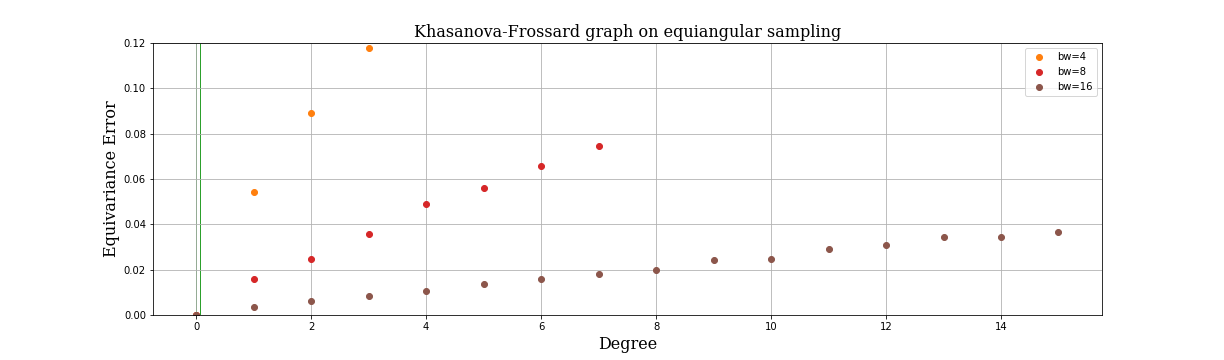
\includegraphics[width=\textwidth]{KhasanovaFrossardgraphonequiangularsampling.png}
	\caption{Equivariance error of the Khasanova-Frossard graph on the equiangular sampling with bandwidth $b=8$ by spherical harmonic degree $\ell$.}
	\label{fig:Equivariance error of the Frossard-Khasanove graph}
\end{figure}

\paragraph{Link with the Laplace-Beltrami Operator}

Given a sampling $x_0, \dots, x_{n-1}$ define $\sigma_i$ to be the patch of the surface of the sphere corresponding to the $i$th point of the sampling, define $A_i$ to be its corresponding area and $d_i$ to be the radius of the smallest ball in $\mathbb R^3$ containing the $i$-th patch. Define $d^{(n)} := \max_{i=0, \dots, n}d_i$ and $A^{(n)}=\max_{i=0, \dots, n}A_i$.

\begin{theorem}
	For a sampling $\mathcal P = \{x_i\in\mathbb S^2\}_{i=0}^{n-1}$ of the sphere that is equi area and such that $d^{(n)} \leq \frac{C}{\sqrt{n}}$, for all $f: \mathbb S^2 \rightarrow \mathbb R$ Lipschitz with respect to the euclidean distance in $\mathbb R^3$, for all $y\in\mathbb S^2$, there exists a sequence $t_n = n^\beta$ such that the rescaled Heat Kernel Graph Laplacian operator $\frac{|\mathbb S^2|}{4\pi t_n}L^t_n$ converges pointwise to the Laplace Beltrami operator on the sphere $\triangle_{\mathbb S^2}$  for $n\to\infty$:
	$$ \lim_{n\to\infty}\frac{|\mathbb S^2|}{4\pi t_n} L_n^{t_n}f(y) =  \triangle_{\mathbb S^2}f(y).$$
	\label{theo:pointwise convergence in the healpix case}
\end{theorem}



\subsection{MATERIAL FROM MARTINO'S MASTER PROJECT}

\todo{
* define a measure of equiv error \\
* show convergence empirically (for Nside up to 1024) \\
* improved upon V1 \\
* no difference in practice (see experiment xx) $\Rightarrow$ NNs are resilient to equiv error \\
}

Take a sampling scheme $V=\{v_i\in\mathbb S^2, i=0, \dots, n\}$ of the sphere, a weighted undirected graph $G(V, E, \mathbf W)$, a signal $f: \mathbb S^2\to\mathbb R$ and its sampled representation $\mathbf f:\ f_i=f(v_i)$. Suppose that there exists a sampling operator $T_V: L^2(\mathbb S^2) \supset F\to \mathbb R^n,\  T_V(f) = \mathbf f$ defined on a suitable subspace $F$ of $L^2(\mathbb S^2)$ such that it is invertible, i.e., we can unambiguously reconstruct the function $f\in F$ from its sampled values $\mathbf f$. The existence of such subspace depends on the sampling scheme $V$, and its characterization is a common problem in signal processing \cite{Driscoll:1994:CFT:184069.184073}. Define the rotation operator $\Lambda(g), g\in SO(3)$: $\Lambda(g) f(\omega) = f\left(g^{-1} \omega\right)$.

We now want to understand how to set the edges and the weights of $G$ such that
\begin{equation} \label{eq:equivariance}
	T \Lambda(g) T^{-1} \Omega_k T f = \Omega_k T \Lambda(g) f,
\end{equation}
i.e., the graph convolution $\Omega_k$ and any rotation $\Lambda(g)$ commute.

Verifying equation (\ref{eq:equivariance}) is really hard in practice, due to the fact that for almost all sampling schemes $V$ it is not known if there exists a space $F$ in which $T$ is invertible. A special case is the \textit{equiangular sampling} scheme where a sampling theorem holds \cite{Driscoll:1994:CFT:184069.184073}, and thus we have a closed form of $T^{-1}$. For sampling schemes where no such sampling theorem is available, there are implementations of discrete SHT to reconstruct a sampled signal $\mathbf f$, thus providing a way to approximate $T^{-1}$. Thanks to this we are able, for a given sampling, a given function $f$, a given rotation $g$, and a given kernel $k$, to compute the \textit{normalized equivariance error}
\begin{equation} \label{eq:equivariance error}
	E_{G}(f, g) = \left(\frac{ \norm {T \Lambda(g) T^{-1} \Omega_k Tf - \Omega_k T \Lambda(g) f}_{L^2(\mathbb R^2)}}{\norm {Tf}_{L^2(\mathbb R^2)}}\right)^2,
\end{equation}
where $T^{-1}$ is substituted with a discrete SHT in case $T$ is not invertible.
A measure of how equivariant a graph is with respect to rotations will then be given by the \textit{mean equivariance error}
\begin{equation} \label{eq:mean equivariance error}
	\overline E_G = \mathbb E_{f, g} \ E_G(f, g).
\end{equation}
In practice the expected value is obtained by averaging over a finite number of random functions and random rotations. The mean equivariance error $\overline E_G$ gives us an indication of how close the graph $G$ is from being equivariant to rotations. Now we state an intuitive concept that explains how to construct rotation invariant graphs, i.e., graphs such that $\overline{E_G}$ is small.
The mean equivariance error $\overline{E_G}$ will be small if the scalar product $\mathbf f^T \mathbf v_{i(\ell, m)}$ well approximates $\hat {f}(\ell,m)$, i.e., the $L^2$ scalar product of the continuous signal $\hat {f}(\ell,m)= \int_{\eta \in \mathbb S^2}f(\eta)Y_\ell^m(\eta)d\mu(\eta)$.

\textit{If $V$ is an equal area sampling scheme}, i.e., the area around each pixel $v_i$ is the same, $\overline{E_G}$ will be small if the graph Laplacian $\mathbf L$ is such that its eigenvectors $\mathbf v_i$ well approximate the eigenfunctions of the Laplace-Beltrami operator $\Delta_{\mathbb S^2}$ evaluated in the points of the sampling scheme, i.e., $\mathbf v_{i(\ell, m)} \approx Y_\ell^m(x_i)$.

In this way we framed the problem of constructing a rotation invariant graph with the more general problem of coming up with a matrix $\mathbf L$ with some specific spectral properties.

\begin{figure}
	\centering
	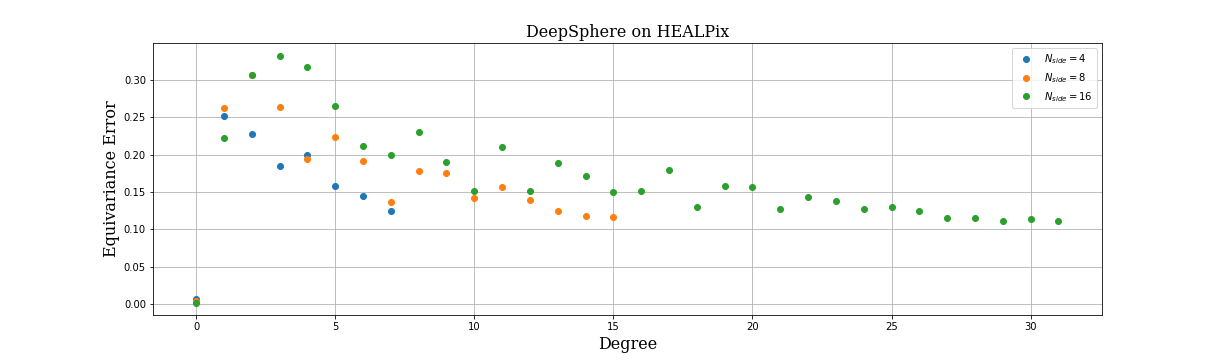
\includegraphics[width=\textwidth]{DeepSphereonHEALPix.png}
	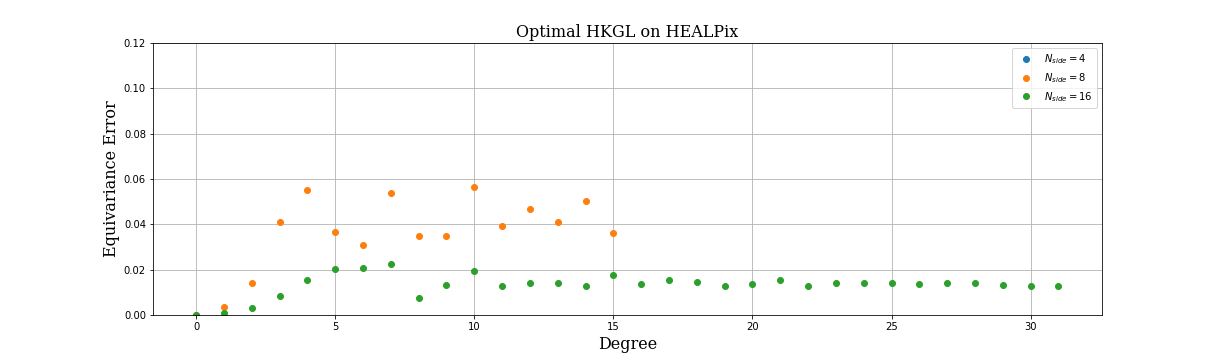
\includegraphics[width=\textwidth]{OptimalHKGLonHEALPix.png}
	\caption{\label{fig:DeepSphere equivariance error}Mean equivariance error of the diffusion filter $\exp(-\Lambda)$ for $G$, $G'$ and the full HKGL, by spherical harmonic degree. Notice the difference in the scale of the y axis for DeepSphere, that reaches errors up to 30\%.}
\end{figure}

\end{document}
